%% Copyright (c) 2002, 2010 Sam Williams
%% Copyright (c) 2010 Richard M. Stallman
%% Permission is granted to copy, distribute and/or modify this
%% document under the terms of the GNU Free Documentation License,
%% Version 1.3 or any later version published by the Free Software
%% Foundation; with no Invariant Sections, no Front-Cover Texts, and
%% no Back-Cover Texts. A copy of the license is included in the
%% file called ``gfdl.tex''.
\chapter{\ifdefined\eng
A Stark Moral Choice
\fi
\ifdefined\chs
道分左右 义无旁支
\fi}
\thispagestyle{empty}
\ifdefined\eng
On September 27, 1983, computer programmers logging on to the Usenet newsgroup net.unix-wizards encountered an unusual message. Posted in the small hours of the morning, 12:30 a.m. to be exact, and signed by \url{rms@mit-oz}, the message's subject line was terse but attention-grabbing. ``New UNIX implementation,'' it read. Instead of introducing a newly released version of Unix, however, the message's opening paragraph issued a call to arms:
\fi

\ifdefined\chs
1983年9月27日,众多计算机用户像往常一样,登录Usenet的net.unix-wizards新闻组。一条不太寻常的消息映入眼帘。这条消息在当天凌晨过后发出来,准确时间是零点三十分。消息来自署名rms@mit-oz的用户。标题甚是简单,却异常乍眼:《重写UNIX系统》(New UNIX implementation)。这个消息并非是介绍新的UNIX发行版,而是更像一篇邀人入伍的檄文,文章开头写道:
\fi

\ifdefined\eng
\begin{quote}
Starting this Thanksgiving I am going to write a complete Unix-compatible software system called GNU (for Gnu's Not Unix), and give it away free to everyone who can use it. Contributions of time, money, programs and equipment are greatly needed.\endnote{See Richard Stallman, ``Initial GNU Announcement'' (September 1983).}
\end{quote}
\fi

\ifdefined\chs
\begin{quote}
这个感恩节假期,我将开始写一个完全的UNIX兼容系统,叫做GNU,意为``GNU's Not Unix(GNU不是UNIX)``。这个系统任何人都可以自由使用。你如果愿意贡献时间,金钱,程序或者设备,我随时欢迎\endnote{参见理查德·斯托曼,《GNU计划初始宣言》,1983年9月}。
\end{quote}
\fi

\ifdefined\eng
To an experienced Unix developer, the message was a mixture of idealism and hubris. Not only did the author pledge to rebuild the already mature Unix operating system from the ground up, he also proposed to improve it in places. The new GNU system, the author predicted, would carry all the usual components -- a text editor, a shell program to run Unix-compatible applications, a compiler, ``and a few other things.''\endnote{\textit{Ibid.}} It would also contain many enticing features that other Unix systems didn't yet offer: a graphic user interface based on the Lisp programming language, a crash-proof file system, and networking protocols built according to MIT's internal networking system.
\fi

\ifdefined\chs
对于UNIX的资深用户来说,这个消息显得太过理想主义,甚至有些自大傲慢。面对已经非常成熟的UNIX系统,这则消息不仅号称要从头克隆一套类似的操作系统,甚至还要在开发过程中改进现有UNIX的设计。这则消息的作者声称,新的GNU系统,会提供各种常用软件,包括文本编辑器,用来执行各种命令和程序的shell,编译器,还有``一些其他的东西\endnote{\textit{同上}}''。除此以外,它还提供很多原本UNIX并不具备的功能,包括一套基于Lisp语言的图形用户界面;一个防崩溃的文件系统;以及一套基于麻省理工学院内部网络系统的网络协议栈。这些都非常吸引眼球。
\fi

\ifdefined\eng
``GNU will be able to run Unix programs, but will not be identical to Unix,'' the author wrote. ``We will make all improvements that are convenient, based on our experience with other operating systems.''
\fi

\ifdefined\chs
``GNU可以运行现有的UNIX程序,但和现有的UNIX并不完全相同,''作者写道:``我们会在开发过程中,融合我们的经验和对其他操作系统的了解,不断改进现有的UNIX系统设计。''
\fi

\ifdefined\eng
Anticipating a skeptical response on some readers' part, the author made sure to follow up his operating-system outline with a brief biographical sketch titled, ``Who am I?'':
\fi

\ifdefined\chs
读者的各种质疑显然早在意料之中,整个消息最后,作者加入了一段《我是谁?》的自我介绍:
\fi

\ifdefined\eng
\begin{quote}
I am Richard Stallman, inventor of the original much-imitated EMACS editor, now at the Artificial Intelligence Lab at MIT. I have worked extensively on compilers, editors, debuggers, command interpreters, the Incompatible Timesharing System and the Lisp Machine operating system. I pioneered terminal-independent display support in ITS. In addition I have implemented one crashproof file system and two window systems for Lisp machines.\endnote{\textit{Ibid.}}
\end{quote}
\fi

\ifdefined\chs
\begin{quote}
我是理查德·斯托曼,EMACS编辑器的作者。如今有很多人都在效仿这个编辑器。现在在麻省理工学院人工智能实验室,我的工作涉及编译器,编辑器,调试器,解释器,还有非兼容分时系统(ITS)以及Lisp机的操作系统。我创造了ITS上早期的独立于各终端硬件的显示技术。我还在Lisp机上实现了一个防崩溃的文件系统,和两个窗口系统\endnote{\textit{同上}}。``
\end{quote}
\fi

\ifdefined\eng
\ifdefined\vone
As fate would have it, Stallman's fanciful GNU Project missed its Thanksgiving launch date. By January, 1984, however, Stallman made good on his promise and fully immersed himself in the world of Unix software development. For a software architect raised on ITS, it was like designing suburban shopping malls instead of Moorish palaces. Even so, building a Unix-like operating system had its hidden advantages. ITS had been powerful, but it also possessed an Achilles' heel: MIT hackers had designed it to take specific advantage of the DEC-built PDP line. When AI Lab administrators elected to phase out the lab's powerful PDP-10 machine in the early 1980s, the operating system that hackers once likened to a vibrant city became an instant ghost town. Unix, on the other hand, was designed for mobility and long-term survival. Originally developed by junior scientists at AT\&T, the program had slipped out under corporate-management radar, finding a happy home in the cash-strapped world of academic computer systems. With fewer resources than their MIT brethren, Unix developers had customized the software to ride atop a motley assortment of hardware systems: everything from the 16-bit PDP-11-a machine considered fit for only small tasks by most AI Lab hackers-to 32-bit mainframes such as the VAX 11/780. By 1983, a few companies, most notably Sun Microsystems, were even going so far as to develop a new generation of microcomputers, dubbed ``workstations,'' to take advantage of the increasingly ubiquitous operating system.
\fi
\ifdefined\vtwo
As fate would have it, Stallman's fanciful GNU Project missed its Thanksgiving launch date. By January, 1984, however, Stallman made good on his promise and fully immersed himself in the world of Unix software development. For a software architect raised on ITS, it was like designing suburban shopping malls instead of Moorish palaces. Even so, building a Unix-like operating system had its hidden advantages. ITS had been powerful, but it also possessed an Achilles' heel: MIT hackers had written it specifically to run on the powerful DEC-built PDP-10 computer. When AI Lab administrators elected to phase out the lab's PDP-10 machine in the early 1980s, the operating system that hackers once likened to a vibrant city became an instant ghost town. Unix, on the other hand, was designed for portability, which made it immune to such dangers. Originally developed by junior scientists at AT\&T, the program had slipped out under corporate-management radar, finding a happy home in the cash-strapped world of academic computer systems. With fewer resources than their MIT brethren, Unix developers had customized the software to ride atop a motley assortment of hardware systems, primarily the 16-bit PDP-11 -- a machine considered fit for only small tasks by most AI Lab hackers -- but later also 32-bit mainframes such as the VAX 11/780. By 1983, a few companies, most notably Sun Microsystems, were developing a more powerful generation of desktop computers, dubbed ``workstations,'' to take advantage of that increasingly ubiquitous operating system on machines comparable in power to the much older PDP-10.
\fi
\fi

\ifdefined\chs
似乎是命中注定一般,斯托曼的GNU系统没能赶在感恩节假期结束前发布。不过斯托曼依旧赶在1984年1月的时候做出了不小的成果,他自己也完全融入到了UNIX软件开发的世界之中。对于这位从ITS世界来的架构师来说,在UNIX中设计软件似乎更像是设计城郊购物中心,而非设计紫禁城皇宫。即便如此,设计成类UNIX系统依旧有它的优势。ITS的确强大,但仍有一处致命缺陷:麻省理工学院的黑客们创造的ITS系统,是专门针对当时强大的DEC PDP-10计算机设计。可到了八十年代,人工智能实验室的管理员决定淘汰掉实验室的PDP-10计算机。当年辉煌一时的ITS系统也因此成了一座无人的鬼城。而UNIX的设计则与此不同。它的设计非常强调移植性,它并不依赖于某个特定硬件环境。因此,面对硬件更替,UNIX则毫无压力。UNIX最初是由当时AT\&T贝尔实验室的几个年轻科学家创造。之后,这套系统被大家纷纷传阅,不断改进。在资金并不富裕的学术界,UNIX系统甚是流行。和麻省理工学院的同僚们不同,UNIX的作者可用的硬件资源非常有限。他们必须把软件设计得可以在各种良莠不齐的硬件上运行无阻。最初是针对PDP-11系统设计,PDP-11是DEC推出的另一种16位计算机。在麻省理工人工智能实验室的黑客们看来,它顶多只能用来跑些小程序。之后,UNIX又陆续开始支持32位计算机,比如VAX11/780。到了1983年,一些公司开始推出更强大的一代被称作``工作站''的桌面计算机。其中以Sun公司产品最为引人注目。这些运行着UNIX的计算机有着更小的体积,却和当年的PDP-10性能相当。
\fi

\ifdefined\vone
\ifdefined\eng
To facilitate this process, the developers in charge of designing the dominant Unix strains made sure to keep an extra layer of abstraction between the software and the machine. Instead of tailoring the operating system to take advantage of a specific machine's resources-as the AI Lab hackers had done with ITS and the PDP-10-Unix developers favored a more generic, off-the-rack approach. Focusing more on the interlocking standards and specifications that held the operating system's many subcomponents together, rather than the actual components themselves, they created a system that could be quickly modified to suit the tastes of any machine. If a user quibbled with a certain portion, the standards made it possible to pull out an individual subcomponent and either fix it or replace it with something better. Simply put, what the Unix approach lacked in terms of style or aesthetics, it more than made up for in terms of flexibility and economy, hence its rapid adoption.\endnote{See Marshall Kirk McKusick, ``Twenty Years of Berkeley Unix,'' \textit{Open Sources} (O'Reilly \& Associates, Inc., 1999): 38.}
\fi

\ifdefined\chs
为了增强可移植能力,负责UNIX开发的程序员在软件和计算机之间,加入了一个抽象层。和人工智能实验室的PDP-10上的ITS系统不同,UNIX并不使用针对某个硬件平台所特有的系统资源进行开发,而是采用了一种更为通用和现成的实现方式。开发者们于是可以放眼全局,集中设计各个组件之间的协调机制,设计组件的接口标准,而不必把精力分散到每个组件的开发和移植上。他们由此创造了一套系统,可以轻易地被移植到各种计算机上。如果某个用户对哪个组件不满意,他们可以按照定义好的接口标准,修改现有组件,甚至重新开发一个同样功能的组件,再把改进的组件放回原位,一切依旧会运行正常。简而言之,抛开美学上的意义不谈,UNIX的设计具备极大的灵活性,这也促进了计算机这个市场的发展,更为UNIX带来了无限生机\endnote{参见马歇尔·柯克·麦库西克(Marshall Kirk McKusick)的文章《伯克利UNIX二十年》,该文收录于《开源软件文集》中。该书中文版已由中国电力出版社出版。}。
\fi

\ifdefined\eng
Stallman's decision to start developing the GNU system was triggered by the end of the ITS system that the AI Lab hackers had nurtured for so long. The demise of ITS had been a traumatic blow to Stallman. Coming on the heels of the Xerox laser printer episode, it offered further evidence that the AI Lab hacker culture was losing its immunity to business practices in the outside world.
\fi

\ifdefined\chs
斯托曼之所以决定开发一套名为GNU的类UNIX系统,是因为人工智能实验室已经停止使用ITS了。而整个实验室的黑客文化,也伴随这ITS的消亡,渐渐分崩离析。这个改变对斯托曼来说,可谓打击重大。施乐公司打印机事件,也从另一个方而证明了,人工智能实验室的黑客文化正渐渐迷失在实验室外的商业世界里。
\fi

\ifdefined\eng
Like the software code that composed it, the roots of ITS' demise stretched way back. Defense spending, long a major font for computer-science research, had dried up during the post-Vietnam years. In a desperate quest for new funds, laboratories and universities turned to the private sector. In the case of the AI Lab, winning over private investors was an easy sell. Home to some of the most ambitious computer-science projects of the post-war era, the lab became a quick incubator of technology. Indeed, by 1980, most of the lab's staff, including many hackers, were dividing its time between Institute and commercial projects.
\fi

\ifdefined\chs
ITS的消亡过程历经了很长时间。在越南战争之后,很多原本可以用于计算机科学研究的国防经费也开始捉襟见肘。为了能够寻求到更多的资金,实验室和大学都开始转向私人领域。就拿人工智能实验室来说,要从一些私人投资者那里争取到资助是非常容易的。作为战后时期很多重要项目的发源地,人工智能实验室很快就成为各种高新技术的孵化器。事实上,到了1980年,包括很多黑客在内的实验室大部分成员都同时参与研究项目与商业项目。
\fi

\ifdefined\eng
What at first seemed like a win-win deal-hackers got to work on the best projects, giving the lab first look at many of the newest computer technologies coming down the pike-soon revealed itself as a Faustian bargain. The more time hackers devoted to cutting-edge commercial projects, the less time they had to devote to general maintenance on the lab's baroque software infrastructure. Soon, companies began hiring away hackers outright in an attempt to monopolize their time and attention. With fewer hackers to mind the shop, programs and machines took longer to fix. Even worse, Stallman says, the lab began to undergo a ``demographic change.'' The hackers who had once formed a vocal minority within the AI Lab were losing membership while ``the professors and the students who didn't really love the [PDP-10] were just as numerous as before.''\endnote{See Richard Stallman (1986).}
\fi

\ifdefined\chs
这一开始看上去是个双赢策略:黑客们可以在最优秀的项目里工作,还可以为实验室带来最新的计算机技术。然而这种行为的弊端也逐渐显露。黑客们投入大量时间去开发前沿的商业软件,而无暇维护实验室的软件系统。很快,各个公司开始把黑客们一个个雇走。随着黑客们的离去,实验室的程序和机器要么没人修,要么也要等上好久才有人打理。理查德·斯托曼说,更糟糕的是,实验室正经历了前所未有的``人事变动''。以前,黑客们虽说人少,却是实验室中很重要的一伙人。如今,黑客几乎绝迹,而``不喜欢PDP-10的教授和学生则依旧那么多\endnote{参见斯托曼在瑞典皇家技术研究所的演讲(1986年10月30日): \url{http://www.gnu.org/philosophy/stallman-kth.html}}。''
\fi

\ifdefined\eng
The breaking point came in 1982. That was the year the lab's administration decided to upgrade its main computer, the PDP-10. Digital, the corporation that manufactured the PDP-10, had discontinued the line. Although the company still offered a high-powered mainframe, dubbed the KL-10, the new machine required a drastic rewrite or ``port'' of ITS if hackers wanted to continue running the same operating system. Fearful that the lab had lost its critical mass of in-house programming talent, AI Lab faculty members pressed for Twenex, a commercial operating system developed by Digital. Outnumbered, the hackers had no choice but to comply.
\fi

\ifdefined\chs
该来的终归躲不过。1982年,人工智能实验室接到通知,要求替换那台已经服役了12年的PDP-11计算机。PDP-11曾是迪吉多公司(Digital Equipment Corporation,简称DEC)出品的16位计算机。在1982年,迪吉多公司的主打产品是Decsystem 20。对于应用程序来说,Decsystem 20和PDP-11兼容。但是如果想要在上面运行ITS这样的操作系统,则需要投入大量劳力,把系统从PDP-11移植到Decsystem 20上。当下的人工智能实验室早已物是人非,实验室中的编程能手几乎都已走光。而实验室中的一些教授则大力鼓吹Twenex系统,它是一款由迪吉多开发的商业操作系统。由于黑客们在人数上处于劣势,只好将就着用Twenex系统。
\fi
\fi

\ifdefined\vtwo
\ifdefined\eng
To facilitate portability, the developers of Unix had put an extra layer of abstraction between the software and the machine. Rather than writing it in the instructions of a specific machine type -- as the AI Lab hackers had done with ITS and the PDP-10 -- Unix developers wrote in a high-level language, called C. Focusing more on the interlocking interfaces and specifications that held the operating system's many subcomponents together, rather than the actual components themselves, they created a system that could be quickly modified to run on any machine. If a user disliked a certain component, the interface specifications made it possible to pull out an individual subcomponent and either fix it or replace it with something better. Simply put, the Unix approach promoted flexibility and economy, hence its rapid adoption.\endnote{See Marshall Kirk McKusick, ``Twenty Years of Berkeley Unix,'' \textit{Open Sources} (O'Reilly \& Associates, Inc., 1999): 38.}
\fi

\ifdefined\chs
为了增强可移植能力,UNIX的开发者在软件和计算机之间,加入了一个抽象层。和人工智能实验室的ITS系统不同,UNIX并非使用特定于某个硬件平台的指令集开发。它的开发者们创造了一种被称为``C语言''的更抽象的编程语言,借此屏蔽了底层的硬件差异。开发者们于是可以放眼全局,集中设计各个组件之间的协调机制,设计组件的接口,而不必把精力分散到每个组件的开发和移植上。他们由此创造了一套系统,可以轻易地被移植到几乎各种计算机上。如果某个用户对哪个组件并不满意,他们可以按照定义好的接口,修改现有组件,甚至重新开发一个同样功能的组件,再把改进的组件放回原位,一切依旧会运行正常。简而言之,UNIX的设计具备极大的灵活性,这也促进了计算机这个市场的发展,更为UNIX带来了无限生机\endnote{参见马歇尔·柯克·麦库西克(Marshall Kirk McKusick)的文章《伯克利UNIX二十年》,该文收录于《开源软件文集》中。该书中文版已由中国电力出版社出版。}。
\fi

\ifdefined\eng
Stallman's decision to start developing the GNU system was triggered by the end of the ITS system that the AI Lab hackers had nurtured for so long. The demise of ITS, and the AI Lab hacker community which had sustained it, had been a traumatic blow to Stallman. If the Xerox laser printer episode had taught him to recognize the injustice of proprietary software, the community's death forced him to choose between surrendering to proprietary software and opposing it.
\fi

\ifdefined\chs
斯托曼之所以决定开发一套名为GNU的类UNIX系统,是因为人工智能实验室已经停止使用ITS了。而整个实验室的黑客文化,也伴随这ITS的消亡,渐渐分崩离析。这个改变对斯托曼来说,可谓打击重大。施乐公司打印机事件,让他意识到了专有软件的不义。而实验室的黑客社区几乎解散,则让斯托曼必须面对抉择:要么在专有软件面前投降,要么起身反抗它。
\fi

\ifdefined\eng
Like the software code that composed it, the roots of ITS' demise stretched way back.  By 1980, most of the lab's hackers were working on developing the Lisp Machine and its operating system.
\fi

\ifdefined\chs
ITS的消亡过程历经了很长时间。1980年的时候,实验室里的大部分黑客都在开发Lisp机(Lisp Machine)和运行其上的操作系统。
\fi

\ifdefined\eng
Created by artificial-intelligence research pioneer John McCarthy, a MIT artificial-intelligence researcher during the late 1950s, Lisp is an elegant language, well-suited for writing complex programs to operate on data with irregular structure. The language's name is a shortened version of LISt Processing. Following McCarthy's departure to the Stanford Artificial Intelligence Laboratory, MIT hackers refined the language into a local dialect dubbed MACLISP. The ``MAC'' stood for Project MAC, the DARPA-funded research project that gave birth to the AI Lab and the Laboratory for Computer Science. Led by AI Lab arch-hacker Richard Greenblatt, the AI Lab hackers during the late 1970s designed a computer specialized for running Lisp efficiently and conveniently, the Lisp Machine, then developed an entire Lisp-based operating system for it.
\fi

\ifdefined\chs
Lisp是一种非常优雅的编程语言。它最初由人工智能领域的先驱,约翰·麦卡锡(John McCarthy)发明。二十世纪五十年代,他曾是麻省理工学院人工智能领域的科学家。他发明的Lisp语言,非常适合编写复杂程序,来处理不具备很好结构的数据。Lisp这个名字来自LISt Processing,即链表处理。之后,约翰·麦卡锡离开了麻省理工学院,去了斯坦福大学的人工智能实验室。麻省理工学院的黑客们则改进了Lisp语言,并创造了一个Lisp方言,名为MACLISP。其中的``MAC'',指的是``MAC项目''。MAC项目是一个由美国国防部高等研究计划局(DARPA)资助的项目。借助这个项目,诞生了如今的人工智能实验室。整个实验室由黑客理查德·格林布拉特(Richard Greenblatt)领导。在七十年代末期,他们设计出了专门用来高效地执行Lisp程序的计算机,命名为Lisp机。接着,开发了一整套基于Lisp的操作系统。
\fi

\ifdefined\eng
By 1980, two rival groups of hackers had formed two companies to manufacture and sell copies of the Lisp Machine.  Greenblatt started Lisp Machines Incorporated.  He planned to avoid outside investment and make a ``hacker company.''  Most of the hackers joined Symbolics, a conventional startup.  In 1982 they entirely ceased to work at MIT.
\fi

\ifdefined\chs
到了1980年,两组互相竞争的黑客各自成立了公司,分别制造和销售Lips机。理查德·格林布拉特成立了``Lisp机公司''(Lisp Machines Incorporated)。他试图避免引入外界的投资,创造一个真正的``黑客公司''。另外一大部分黑客们,则加入了名为Symbolics的传统创业公司。到了1982年,这些黑客则完全放下了在麻省理工学院的工作。
\fi

\ifdefined\eng
With few hackers left to mind the shop, programs and machines took longer to fix -- or were not fixed at all.  Even worse, Stallman says, the lab began to undergo a ``demographic change.'' The hackers who had once formed a vocal minority within the AI Lab were almost gone while ``the professors and the students who didn't really love the [PDP-10] were just as numerous as before.''\endnote{See Richard Stallman (1986).}
\fi

\ifdefined\chs
随着黑客们的离去,实验室的程序和机器要么没人修,要么也要等上好久才有人打理。理查德·斯托曼说,更糟糕的是,实验室正经历了前所未有的``人事变动''。以前,黑客们虽说人少,却是实验室中很重要的一伙人。如今,黑客几乎绝迹,而``不喜欢PDP-10的教授和学生则依旧那么多\endnote{参见斯托曼在瑞典皇家技术研究所的演讲(1986年10月30日): \url{http://www.gnu.org/philosophy/stallman-kth.html}}。''
\fi

\ifdefined\eng
In 1982, the AI Lab received the replacement for its main computer, the PDP-10, which was over 12 years old. Digital's current model, the Decsystem 20, was compatible for user programs but would have required a drastic rewrite or ``port'' of ITS if hackers wanted to continue running the same operating system. Fearful that the lab had lost its critical mass of in-house programming talent, AI Lab faculty members pressed for Twenex, a commercial operating system developed by Digital. Outnumbered, the hackers had no choice but to comply.
\fi

\ifdefined\chs
1982年,人工智能实验室接到通知,要求替换那台已经服役了12年的PDP-11计算机。PDP-11曾是迪吉多公司(Digital Equipment Corporation,简称DEC)出品的16位计算机。在1982年,迪吉多公司的主打产品是Decsystem 20。对于应用程序来说,Decsystem 20和PDP-11兼容。但是如果想要在上面运行ITS这样的操作系统,则需要投入大量劳力,把系统从PDP-11移植到Decsystem 20上。当下的人工智能实验室早已物是人非,实验室中的编程能手几乎都已走光。而实验室中的一些教授则大力鼓吹Twenex系统,它是一款由迪吉多开发的商业操作系统。由于黑客们在人数上处于劣势,只好将就着用Twenex系统。
\fi

\ifdefined\eng
\begin{figure}[ht] \centering
  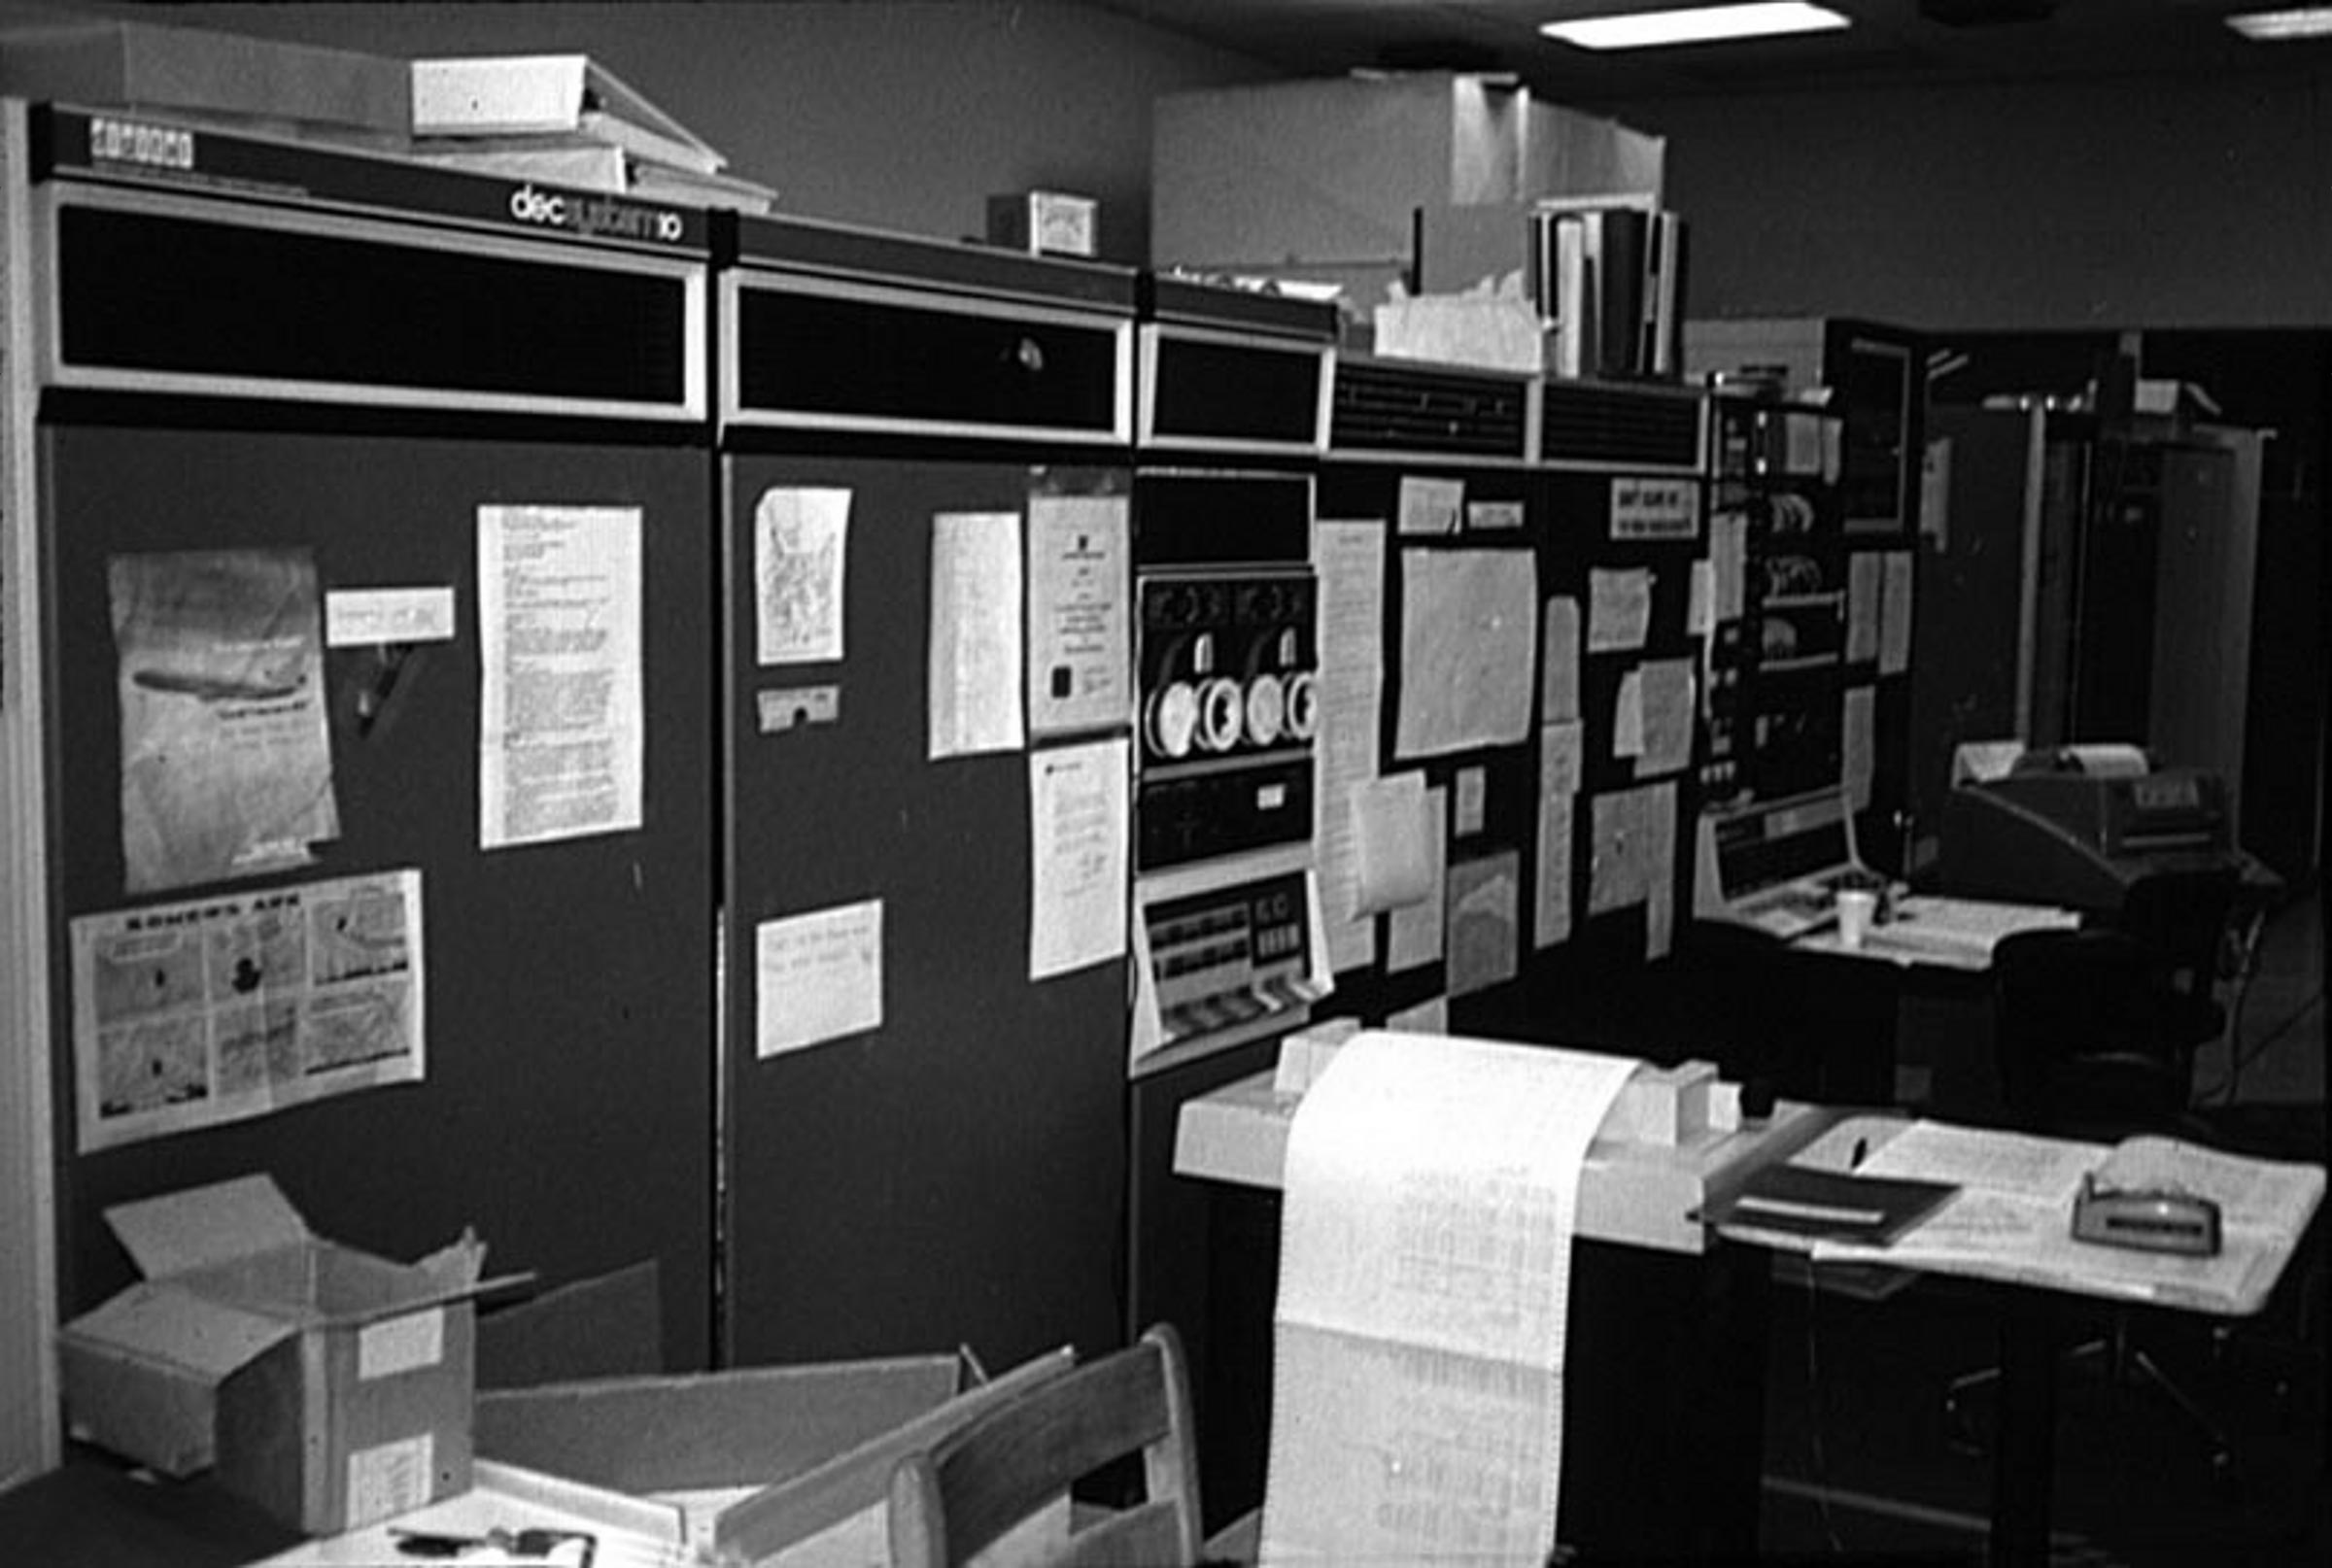
\includegraphics[width=\textwidth]{KL10_1979}
  \caption{PDP-10 processor with KL-10 (a PDP-10 similar to that of the AI Lab), Stanford Artificial Intelligence Laboratory, 1979.}
\end{figure}
\fi

\ifdefined\chs
\begin{figure}[ht] \centering
  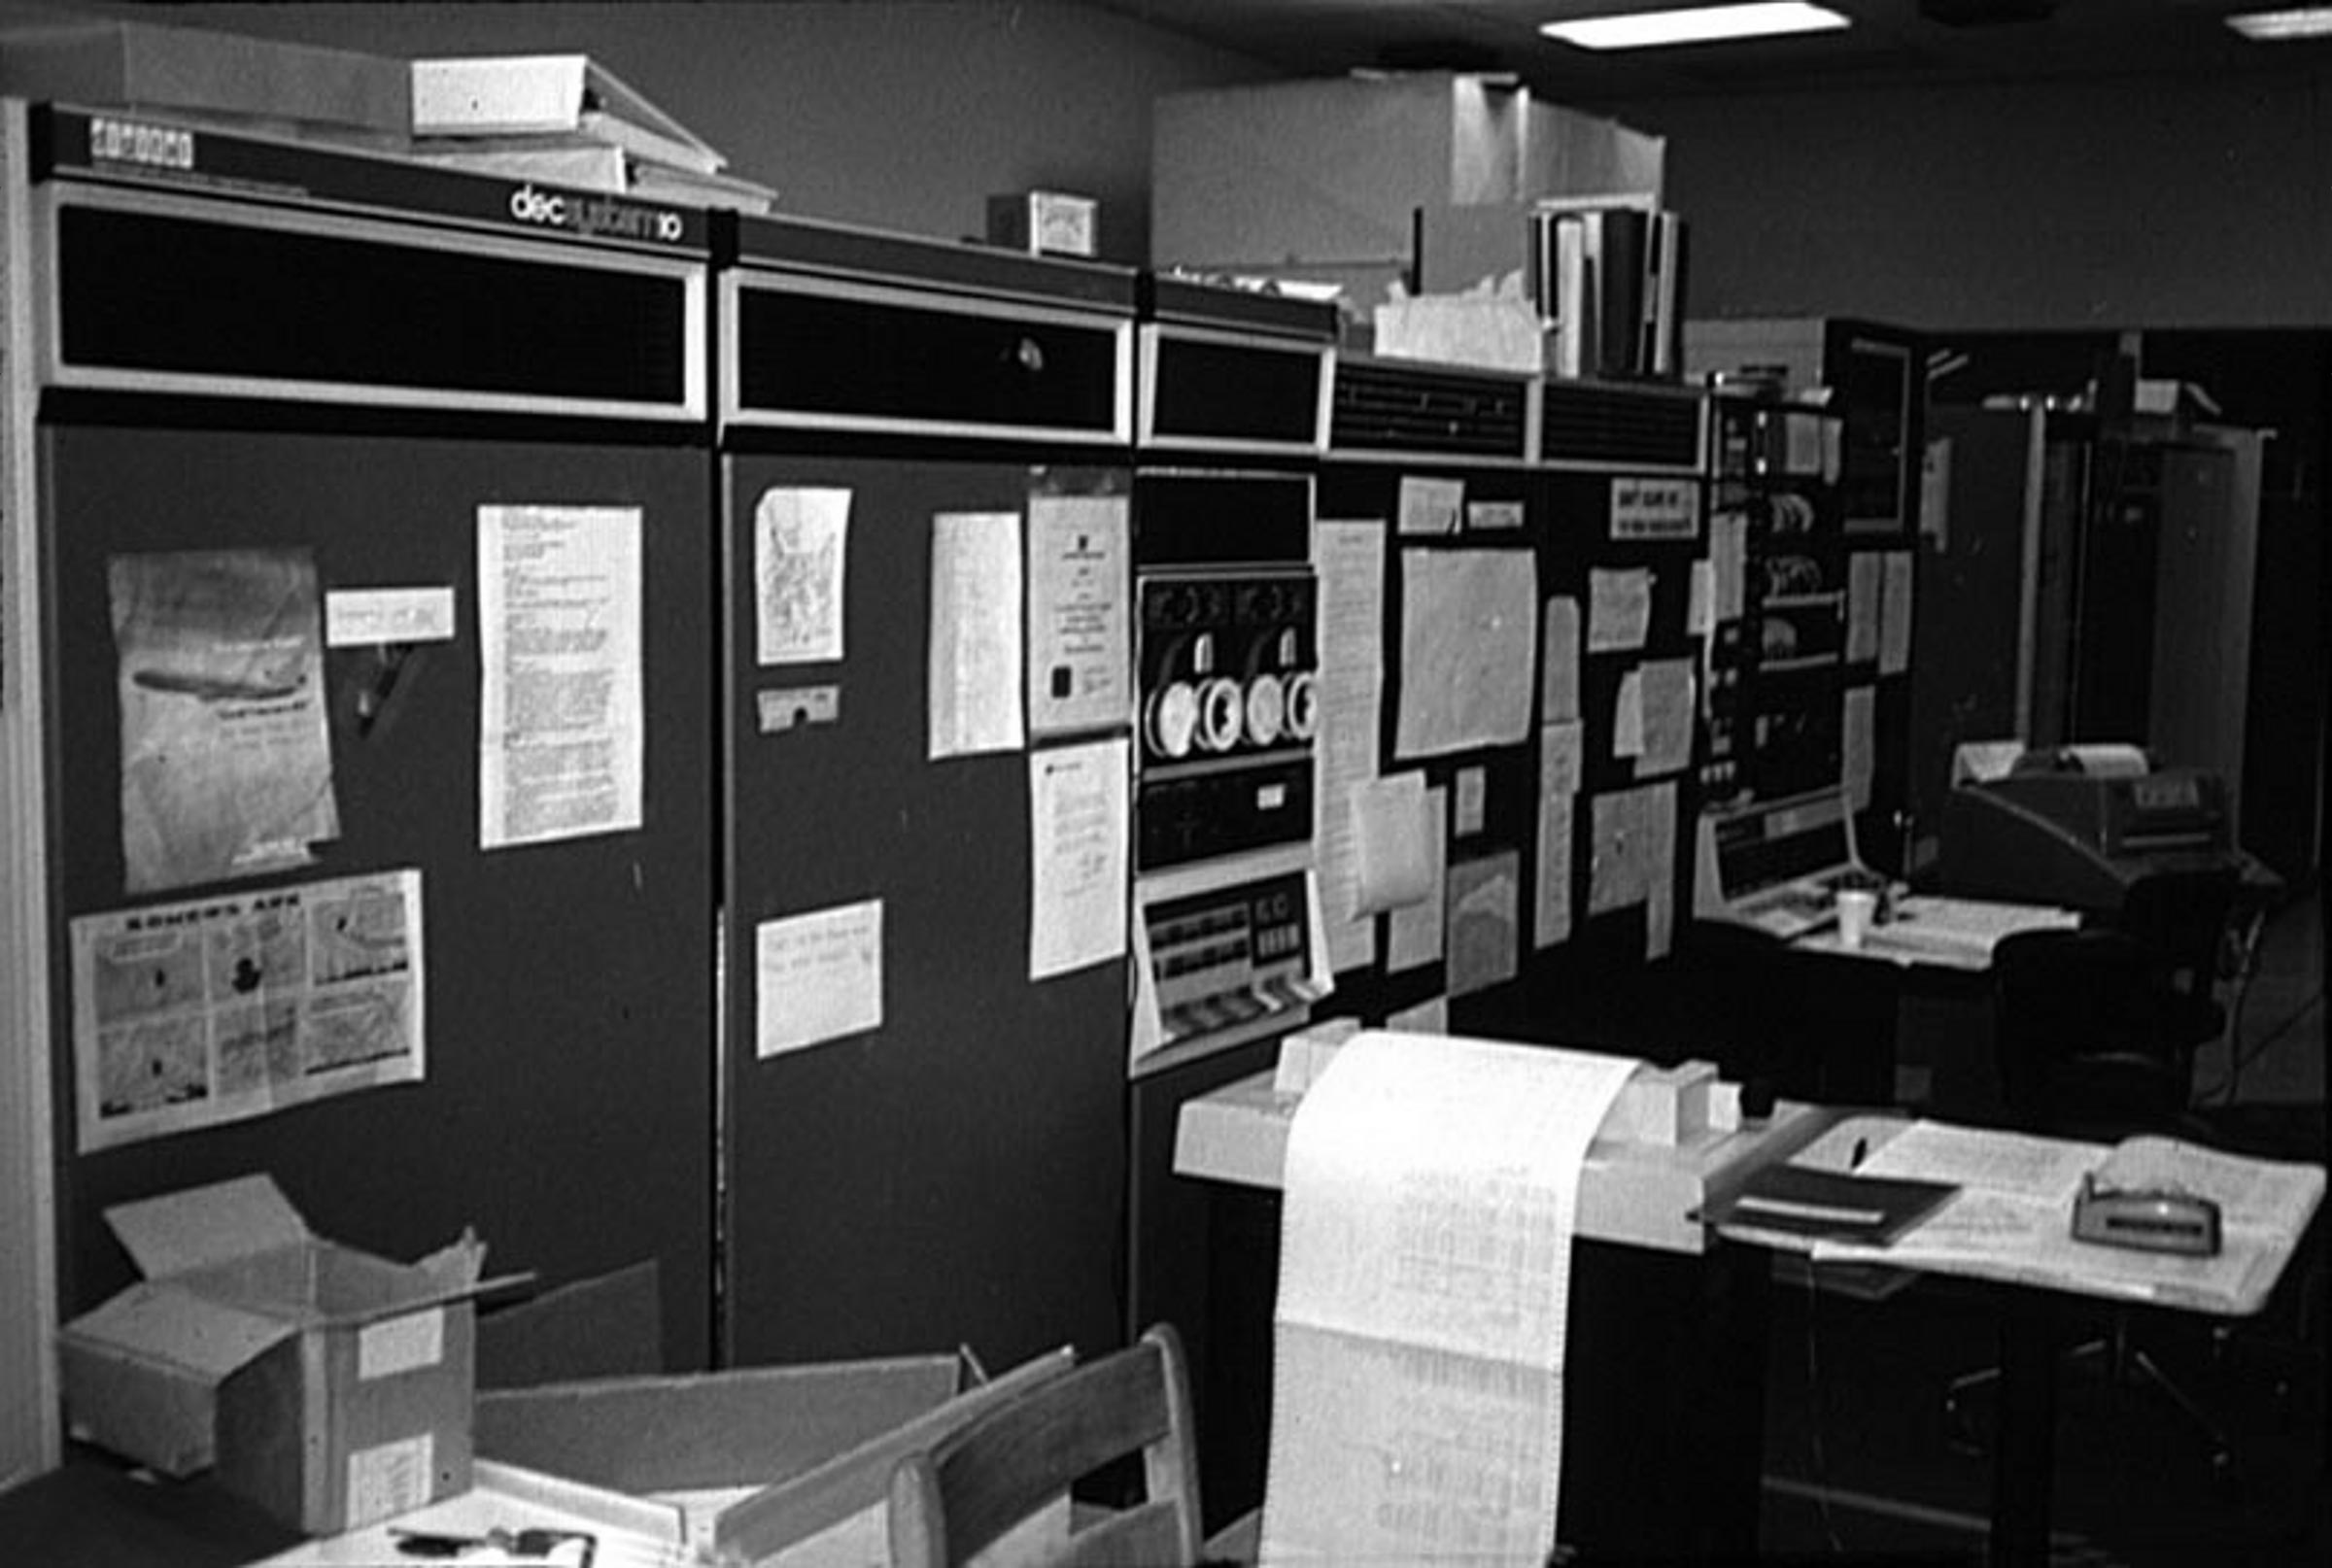
\includegraphics[width=\textwidth]{KL10_1979}
  \caption{PDP-10与KL-10。图片拍摄地点为斯坦福大学人工智能实验室,摄于1979年。}
\end{figure}
\fi
\fi

\ifdefined\eng
``Without hackers to maintain the system, [faculty members] said, `We're going to have a disaster; we must have commercial software,'\hspace{0.01in}'' Stallman would recall a few years later. ``They said, `We can expect the company to maintain it.' It proved that they were utterly wrong, but that's what they did.''\endnote{\textit{Ibid.}}
\fi

\ifdefined\chs
几年之后,斯托曼回忆起那时的情景:``那些教授们说:`没有足够的黑客们来维护ITS系统,我们将会面临各种灾难。要避免这些发生,我们只能投靠商业软件。我们可以让商业公司来提供维护。'后来的事实证明,他们的这番论调大错特错。可当时他们的确这么做了\endnote{\textit{同上}}。''
\fi

\ifdefined\eng
At first, hackers viewed the Twenex system as yet another authoritarian symbol begging to be subverted. The system's name itself was a protest. Officially dubbed TOPS-20 by DEC, it was \ifdefined\vtwo named\fi as a successor to TOPS-10, a \ifdefined\vone commerical \fi\ifdefined\vtwo proprietary \fi operating system DEC \ifdefined\vone marketed \fi\ifdefined\vtwo distributed \fi for the PDP-10. \ifdefined\vone Bolt Beranek Newman had deveoped an improved version, dubbed Tenex, which TOPS-20 drew upon.\endnote{Multiple sources: see Richard Stallman interview, Gerald Sussman email, and \textit{Jargon File 3.0.0} at \url{http://catb.org/jargon/html/T/TWENEX.html}.} Stallman, \fi\ifdefined\vtwo But TOPS-20 was not based on TOPS-10.  It was derived from the Tenex system which Bolt Beranek Newman had developed for the PDP-10.\endnote{Multiple sources: see Richard Stallman interview, Gerald Sussman email, and \textit{Jargon File 3.0.0} at \url{http://catb.org/jargon/html/T/TWENEX.html}.} Stallman, \fi the hacker who coined the Twenex term, says he came up with the name as a way to avoid using the TOPS-20 name. ``The system was far from tops, so there was no way I was going to call it that,'' Stallman recalls. ``So I decided to insert a `w' in the Tenex name and call it Twenex.''
\fi

\ifdefined\chs
一开始,黑客们觉得Twenex只不过又是一个专制的标志。和之前那些专制标志一样,只要把它推翻,就万事大吉了。这个系统从名字看,就像是对黑客们的挑衅:迪吉多公司对这个系统的官方名字是TOPS-20,意为``顶尖20''。它是TOPS-10的后继产品,而TOPS-10则是迪吉多当年给PDP-10配备的标准系统。不过TOPS-20并非是在TOPS-10基础上做的开发。它的主要代码都继承自BBN公司(Bolt, Beranek and Newman)为PDP-10开发的Tenex系统\endnote{参见《黑话词典3.0.0》 \url{http://catb.org/jargon/html/T/TWENEX.html}}。斯托曼则由此把TOPS-20称作Twenex,因为他实在不想用TOPS-20这个名字。他说:``这个系统可根本算不上`顶尖',我说什么也不会这么夸它。所以我在Tenex里添了个字母w,把它叫做Twenex。''
\fi

\ifdefined\eng
The machine that ran the Twenex/TOPS-20 system had its own derisive nickname: Oz. According to one hacker legend, the machine got its nickname because it required a smaller PDP-11 machine to power its terminal. One hacker, upon viewing the KL-10-PDP-11 setup for the first time, likened it to the wizard's bombastic onscreen introduction in the Wizard of Oz. ``I am the great and powerful Oz,'' the hacker intoned. ``Pay no attention to the PDP-11 behind that console.''\endnote{See \url{http://www.as.cmu.edu/~geek/humor/See_Figure_1.txt}.}
\fi

\ifdefined\chs
在黑客界,人们把跑着TOPS系统的Decsystem计算机戏称作Oz,意为``奥兹国''。奥兹国这名字源自《绿野仙踪》这部小说。因为在黑客界,人们都说这样一台计算机需要有个PDP-11作为终端机才能运行。于是,人们看到这台计算机连着PDP-11作为终端,就不禁想到了《绿野仙踪》中那位吹牛皮的奥兹国大法师。黑客们常戏谑道:``我是伟大全能的奥兹国大法师!我可没看到身后那台PDP-11。\endnote{参见\url{http://www.as.cmu.edu/~geek/humor/See_Figure_1.txt}。}''
\fi

\ifdefined\eng
If hackers laughed when they first encountered the KL-10, their laughter quickly died when they encountered Twenex. Not only did Twenex boast built-in security, but the system's software engineers had designed the tools and applications with the security system in mind. What once had been a cat-and-mouse game over passwords in the case of the Laboratory for Computer Science's security system, now became an out-and-out battle over system management. System administrators argued that without security, the Oz system was more prone to accidental crashes. Hackers argued that crashes could be better prevented by overhauling the source code. Unfortunately, the number of hackers with the time and inclination to perform this sort of overhaul had dwindled to the point that the system-administrator argument prevailed.
\fi

\ifdefined\chs
黑客们当年第一次看到Decsystem的时候也许还会借机嘲笑两句,可很快他们就在Twenex面前笑不起来了。Twenex系统增进了系统的安全强度,而且Twenex上的软件也都考虑了各种安全措施。当年,黑客们试图避免设置任何密码和安全设施,那些行为就好像在和管理员玩猫捉老鼠的游戏。而如今,他们面对的,则是一场彻头彻尾的战斗了。系统管理员辩解说,如果没有这些安全设施,Oz系统就随时都会面临崩溃。而黑客们则辩解说,避免崩溃的最好办法,就是公开程序的源代码。遗憾的是,黑客人数上不占优,而且大多数黑客也逐渐失去了当年的那份果断。最终,系统管理员还是胜利了。
\fi

\ifdefined\vtwo
\ifdefined\eng
The initial policy was that any lab member could have the ``wheel privilege'' to bypass security restrictions.  But anyone who had the ``wheel privilege'' could take it away from anyone else, who would then be powerless to restore it.  This state of affairs tempted a small group of hackers to try to seize total control by canceling the ``wheel privilege'' for all but themselves.
\fi

\ifdefined\chs
一开始的政策是,任何一个人工智能实验室的成员,都拥有一个``特权车服务''(wheel privilege),可以用来绕过系统的安全限制。可是,任何有``特权车''的人,都有权吊销别人的``特权车''。这样一来,就促使一小撮黑客总是尝试吊销其他人的特权,借此掌控全局。
\fi
\fi

\ifdefined\eng
\ifdefined\vone
Cadging passwords and deliberately crashing the system in order to glean evidence from the resulting wreckage, Stallman successfully foiled the system administrators' attempt to assert control. After one foiled ``\textit{coup d'etat},'' Stallman issued an alert to the entire AI staff.\endnote{See Richard Stallman (1986).}
\fi
\ifdefined\vtwo
Cadging passwords, and applying the debugger during startup, Stallman successfully foiled these attempts. After the second foiled ``\textit{coup d'état},'' Stallman issued an alert to all the AI Lab personnel.\endnote{See Richard Stallman (1986).}
\fi
\fi

\ifdefined\chs
见得此状,斯托曼破解了密码,利用开机时的调试器,成功破坏了几个这样企图夺权的阴谋。在第二轮``政变''之后,斯托曼向全体人工智能实验室的人发出了警告信\endnote{参见斯托曼在瑞典皇家技术研究所的演讲(1986年10月30日): \url{http://www.gnu.org/philosophy/stallman-kth.html}}。
\fi

\ifdefined\eng
``There has been another attempt to seize power,'' Stallman wrote. ``So far, the aristocratic forces have been defeated.'' To protect his identity, Stallman signed the message ``Radio Free OZ.''
\fi

\ifdefined\chs
信中写道:``还有另外一波强大的力量,企图剥夺我们的权利。不过现在,这些官僚们已经暂时被我们打败了。''这是封匿名信,信底的签名是``自由奥兹国电台''。
\fi

\ifdefined\eng
The disguise was a thin one at best. By 1982, Stallman's aversion to passwords and secrecy had become so well known that users outside the AI Laboratory were using his account \ifdefined\vone as a stepping stone to the ARPAnet, the \fi\ifdefined\vtwo\ from around the ARPAnet -- the \fi research-funded computer network that would serve as a foundation for today's Internet. One such ``tourist'' during the early 1980s was Don Hopkins, a California programmer who learned through the hacking grapevine that all an outsider needed to do to gain access to MIT's vaunted ITS system was to log in under the initials RMS and enter the same three-letter monogram when the system requested a password.
\fi

\ifdefined\chs
不过,所谓的匿名信并没把斯托曼挡在幕后。到了1982年,斯托曼关于密码和安全设施的抗议早就内外闻名。以至于有不少人工智能实验室以外的人,通过ARPAnet网络,使用斯托曼的登录账号,访问人工智能实验室的计算机。他们当初使用的ARPAnet,是如今互联网的雏形。它曾是一个研究项目,旨在构造一个大型计算机网络。这个网络之后不断发展,最终成了今天大家见到的互联网。唐·霍普金斯(Don Hopkins)在八十年代是加利福尼亚州的一名程序员,他当年就曾利用斯托曼的账号访问人工智能实验室的计算机。他当年从黑客圈的小道消息里听说,想要使用麻省理工学院大名鼎鼎的ITS系统,只需要使用一个简单的用户名和密码登录就可以:用户名,RMS;密码,RMS。
\fi

\ifdefined\eng
``I'm eternally grateful that MIT let me and many other people use their computers for free,'' says Hopkins. ``It meant a lot to many people.''
\fi

\ifdefined\chs
霍普金斯说:``麻省理工学院让我和很多其他的人免费使用他们的计算机,这让我受益终生。这在当时,对大家来说可是份厚礼。''
\fi

\ifdefined\eng
\ifdefined\vone
This so-called ``tourist'' policy, which had been openly tolerated by MIT management during the ITS years,\endnote{See ``MIT AI Lab Tourist Policy.'' \url{http://catalog.com/hopkins/text/tourist-policy.html}} fell by the wayside when Oz became the lab's primary link to the ARPAnet. At first, Stallman continued his policy of repeating his login ID as a password so outside users could follow in his footsteps. Over time, however, the Oz's fragility prompted administrators to bar outsiders who, through sheer accident or malicious intent, might bring down the system. When those same administrators eventually demanded that Stallman stop publishing his password, Stallman, citing personal ethics, refused to do so and ceased using the Oz system altogether.\endnote{See Richard Stallman (1986).}
\fi
\ifdefined\vtwo
This so-called ``tourist'' policy, which had been openly tolerated by MIT management during the ITS years,\endnote{See ``MIT AI Lab Tourist Policy,'' \url{http://www.art.net/~hopkins/Don/text/tourist-policy.html}.} fell by the wayside when Oz became the lab's primary link to the ARPAnet. At first, Stallman continued his policy of repeating his login ID as a password so outside users could have access through his account. Over time, however, Oz's fragility prompted administrators to bar outsiders who, through sheer accident or malicious intent, might bring down the system. When those same administrators eventually demanded that Stallman stop publishing his password, Stallman, citing personal ethics, instead ceased using the Oz system altogether.\endnote{See Richard Stallman (1986).}
\fi
\fi

\ifdefined\chs
这种允许``游客''的政策,在ITS时代还能被麻省理工学院的管理人员容忍\endnote{参见《麻省理工学院人工智能实验室游客守则》 \url{http://www.art.net/~hopkins/Don/text/tourist-policy.html}}。可等到Oz成为实验室连接ARPAnet的主节点后,这行为就被逐渐禁止了。一开始,斯托曼依旧使用原来简单的用户名和密码,这样外部人员还是可以访问实验室的计算机。但是脆弱的Oz禁不起这么折腾,很快管理员就禁止了外部人员的访问。因为有些访客会有意无意地把整个系统搞垮。再后来,管理员们严重警告了斯托曼公开用户名和密码的行为。对此,斯托曼并没有放弃使用Oz系统,而是在回应中强调了自己的底线\endnote{参见理查德·斯托曼在瑞典皇家技术研究所的演讲(1986年10月30日): \url{http://www.gnu.org/philosophy/stallman-kth.html}}。
\fi

\ifdefined\eng
``[When] passwords first appeared at the MIT AI Lab I [decided] to follow my belief that there should be no passwords,'' Stallman would later say. ``Because I don't believe that it's really desirable to have security on a computer, I shouldn't be willing to help uphold the security regime.''\endnote{\textit{Ibid.}}
\fi

\ifdefined\chs
斯托曼之后说:``当年人工智能实验室第一次要求设置密码,我依旧坚持自己的原则:计算机上不该有密码。我也因此坚决不会帮助他们维护一个充满安全设施的计算机系统。''\endnote{\textit{同上}}
\fi

\ifdefined\eng
\ifdefined\vone
Stallman's refusal to bow before the great and powerful Oz symbolized the growing tension between hackers and AI Lab management during the early 1980s. This tension paled in comparison to the conflict that raged within the hacker community itself. By the time the KL-10 arrived, the hacker community had already divided into two camps. The first centered around a software company called Symbolics, Inc. The second centered around Symbolics chief rival, Lisp Machines, Inc. (LMI). Both companies were in a race to market the Lisp Machine, a device built to take full advantage of the Lisp programming language.
\fi
\ifdefined\vtwo
Stallman's refusal to bow before the great and powerful Oz symbolized the growing tension between hackers and AI Lab management during the early 1980s. This tension paled in comparison to the conflict that raged within the hacker community itself. By the time the Decsystem 20 arrived, the hacker community was divided into two camps, LMI and Symbolics.
\fi
\fi

\ifdefined\chs
\ifdefined\vone
八十年代早期,斯托曼的这次抗议,标志着黑客和系统管理员之间的矛盾进一步升级。不过随着时间的流逝,这种紧张关系反而被黑客圈子内部的矛盾逐渐取代。在KL-10来到实验室的时候,实验室的黑客圈子已经俨然分成了两派。一派主要围绕一家名为Symbolics的商业软件公司,另一派则围绕Symbolics的对手公司Lisp Machines (LMI)。这两家公司在Lisp机的市场竞争中不分上下,这种Lisp机是以Lisp编程语言为基础构建的。
\fi
\ifdefined\vtwo
八十年代早期,斯托曼的这次抗议,标志着黑客和系统管理员之间的矛盾进一步升级。不过随着时间的流逝,这种紧张关系反而被黑客圈子内部的矛盾逐渐取代。在Decsystem 20来到实验室的时候,实验室的黑客圈子已经俨然分成了两派:LMI派和Symbolics派。
\fi
\fi

\ifdefined\vone
\ifdefined\eng
Created by artificial-intelligence research pioneer John McCarthy, a MIT artificial-intelligence researcher during the late 1950s, Lisp is an elegant language well-suited for programs charged with heavy-duty sorting and processing. The language's name is a shortened version of LISt Processing. Following McCarthy's departure to the Stanford Artificial Intelligence Laboratory, MIT hackers refined the language into a local dialect dubbed MACLISP. The ``MAC'' stood for Project MAC, the DARPA-funded research project that gave birth to the AI Lab and the Laboratory for Computer Science. Led by AI Lab arch-hacker Richard Greenblatt, AI Lab programmers during the 1970s built up an entire Lisp-based operating system, dubbed the Lisp Machine operating system. By 1980, the Lisp Machine project had generated two commercial spin-offs. Symbolics was headed by Russell Noftsker, a former AI Lab administrator, and Lisp Machines, Inc., was headed by Greenblatt.
\fi

\ifdefined\chs
Lisp是一种非常优雅的编程语言。它最初由人工智能领域的先驱,约翰·麦卡锡(John McCarthy)发明。二十世纪五十年代,他曾是麻省理工学院人工智能领域的科学家。他发明的Lisp语言,非常适合编写复杂程序,来处理不具备很好结构的数据。Lisp这个名字来自LISt Processing,即链表处理。之后,约翰·麦卡锡离开了麻省理工学院,去了斯坦福大学的人工智能实验室。麻省理工学院的黑客们则改进了Lisp语言,并创造了一个Lisp方言,名为MACLISP。其中的``MAC'',指的是``MAC项目''。MAC项目是一个由美国国防部高等研究计划局(DARPA)资助的项目。借助这个项目,诞生了如今的人工智能实验室。整个实验室由黑客理查德·格林布拉特(Richard Greenblatt)领导。在七十年代末期,他们设计出了专门用来高效地执行Lisp程序的计算机,命名为Lisp机。接着,开发了一整套基于Lisp的操作系统。到了1980年,由Lisp机项目产生了两家商业公司:由人工智能实验室的前主管,罗素·诺夫斯科(Russell Noftsker)创立的Symbolics公司;和理查德·格林布拉特创立的``Lisp机公司''(Lisp Machines Incorporated),即LMI。
\fi

\ifdefined\eng
The Lisp Machine software was hacker-built, meaning it was owned by MIT but available for anyone to copy as per hacker custom. Such a system limited the marketing advantage of any company hoping to license the software from MIT and market it as unique. To secure an advantage, and to bolster the aspects of the operating system that customers might consider attractive, the companies recruited various AI Lab hackers and set them working on various components of the Lisp Machine operating system outside the auspices of the AI Lab.
\fi

\ifdefined\chs
Lisp机的软件系统本身是黑客创造的。它的版权归麻省理工学院所有,但按照黑客传统,任何人都可以获得源代码,复制或修改。然而,这种自由分享的方式却让商业公司很是烦恼:公司的产品无法在市场中显得独一无二,也就少了商机。为了获取优势,吸引用户,两家公司开始从人工智能实验室里挖走黑客。它们把黑客们安排在自己公司里,让他们的代码不再流入人工智能实验室。
\fi

\ifdefined\eng
The most aggressive in this strategy was Symbolics. By the end of 1980, the company had hired 14 AI Lab staffers as part-time consultants to develop its version of the Lisp Machine. Apart from Stallman, the rest signed on to help LMI.\endnote{See H. P. Newquist, \textit{The Brain Makers: Genius, Ego, and Greed in the Quest for Machines that Think} (Sams Publishing, 1994): 172.}
\fi

\ifdefined\chs
在Symbolics和LMI两家公司里,Symbolics挖人的行为相比更加激进。八十年代末期,这家公司已经吸纳了人工智能实验室的14位黑客作为兼职顾问,负责开发他们的Lisp机。剩下的黑客们,除了斯托曼以外,则都在LMI公司就职。\endnote{参见H. P. 纽奎斯特 (H. P. Newquist)所著的《大脑创作家》(The Brain Maker)第172页,Sams Publishing,1984}
\fi
\fi

\ifdefined\vtwo
\ifdefined\eng
Symbolics, with its outside investment, recruited various AI Lab hackers and set some of them working on improving parts of the Lisp Machine operating system outside the auspices of the AI Lab. By the end of 1980, the company had hired 14 AI Lab staffers as part-time consultants to develop its version of the Lisp Machine. The remaining few, apart from Stallman, worked for LMI.\endnote{See Steve Levy, \textit{Hackers}, page 423.}  Stallman, preferring the unpressured life at the AI Lab and not wishing to take a side, chose to join neither company.
\fi

\ifdefined\chs
LMI和Symbolics分别是两家做Lisp机的计算机公司。Symbolics得到了一些外部的投资,它招募了很多人工智能实验室的黑客,把其中的一部分黑客安排去改进Symbolics的Lisp机的操作系统。八十年代末期,这家公司已经吸纳了人工智能实验室的14位黑客作为兼职顾问,负责开发他们的Lisp机。剩下的黑客们,除了斯托曼以外,则都在LMI公司就职\endnote{参见史蒂芬·李维(Steven Levy),《黑客》(1984年,美国企鹅出版社),第423页。}。斯托曼则更享受人工智能实验室里没有压力的工作环境,更不想把自己划进哪个阵营。所以他哪个公司都没加入。
\fi
\fi

\ifdefined\eng
\ifdefined\vone
At first, Stallman accepted both companies' attempt to commercialize the Lisp machine, even though it meant more work for him. Both licensed the Lisp Machine OS source code from MIT, and it was Stallman's job to update the lab's own Lisp Machine to keep pace with the latest innovations. Although Symbolics' license with MIT gave Stallman the right to review, but not copy, Symbolics' source code, Stallman says a ``gentleman's agreement'' between Symbolics management and the AI Lab made it possible to borrow attractive snippets in traditional hacker fashion.
\fi
\ifdefined\vtwo
At first, the other hackers continued spending some of their time at MIT, and contributed to MIT's Lisp Machine operating system. Both LMI and Symbolics had licensed this code from MIT. The license required them to return their changes to MIT, but did not require them to let MIT redistribute these changes.  However, through 1981 they adhered to a gentleman's agreement to permit that, so all their system improvements were included in the MIT version and thus shared with all Lisp Machine users. This situation allowed those still at MIT to remain neutral.
\fi
\fi

\ifdefined\chs
\ifdefined\vone
一开始,斯托曼倒也接受了Lisp机商业化的行为——这无非就是意味着他得多承担些实验室的活,不过斯托曼也没抱怨什么。LMI和Symbolics的Lisp机操作系统都是从麻省理工学院得到的授权,从人工智能实验室的Lisp机操作系统上衍生而来。斯托曼当年的任务是继续开发实验室的Lisp机系统,让它能与最新的研究成果同步。Symbolics公司允许斯托曼查看该公司Lisp操作系统的源代码,但是禁止拷贝。斯托曼说,当年Symbolics和人工智能实验室有个``君子协定'':他们允许实验室在自己的操作系统中,实现Symbolics公司的操作系统中的类似功能,并且允许实验室继续按照黑客的传统发布实验室开发的代码。
\fi
\ifdefined\vtwo
一开始,这些在公司干活的黑客们还会抽出些时间,在麻省理工学院继续做些工作,也会给麻省理工学院的Lisp机的操作系统贡献些代码。LMI和Symbolics的Lisp机操作系统都是从麻省理工学院的Lisp机操作系统上衍生而来。在使用许可证上,麻省理工学院要求两家公司必须允许麻省理工学院使用它们的操作系统。但是,这两家公司可以禁止麻省理工学院再发布他们的产品。不过,1981年间,两家公司之间倒是有个不成文的君子协议,他们都允许麻省理工学院使用并再发布两家公司的代码。这样,麻省理工学院的Lisp机操作系统就包含了来自外部公司的各种改进,而基于许可证,改进后的系统代码又可以继续流入各家公司。这相当于公司之间可以共享代码。如此,那些依旧在麻省理工学院工作的黑客们,就可以继续保持中立。
\fi
\fi

\ifdefined\eng
\ifdefined\vone
On March 16, 1982, a date Stallman remembers well because it was his birthday, Symbolics executives decided to end this gentlemen's agreement. The move was largely strategic. LMI, the primary competition in the Lisp Machine marketplace, was essentially using a copy of the AI Lab Lisp Machine. Rather than subsidize the development of a market rival, Symbolics executives elected to enforce the letter of the license. If the AI Lab wanted its operating system to stay current with the Symbolics operating system, the lab would have to switch over to a Symbolics machine and sever its connection to LMI.
\fi
\ifdefined\vtwo
On March 16, 1982, a date Stallman remembers well because it was his birthday, Symbolics executives ended the gentleman's agreement. The motive was to attack LMI. LMI had fewer hackers, and fewer staff in general, so the Symbolics executives thought that LMI was getting the main benefit of sharing the system improvements.  By ending the sharing of system code, they hoped to wipe out LMI.  So they decided to enforce the letter of the license.  Instead of contributing their improvements to the MIT version of the system, which LMI could use, they provided MIT with a copy of the Symbolics version of the system for users at MIT to run.  Anyone using it would provide the service of testing only to Symbolics, and if he made improvements, most likely they too would only be useful for Symbolics.
\fi
\fi

\ifdefined\chs
\ifdefined\vone
1982年3月16日,斯托曼清晰地记得这一天,那是他的生日。在这一天,Symbolics的主管们决定不再遵循当初那份君子协议。LMI是Symbolics的直接竞争对手,它们使用的操作系统也是来自于人工智能实验室,而实验室的操作系统则是随时更新,且包含Symbolics系统最新特性的。Symbolics于是决心彻查人工智能实验室Lisp操作系统的代码,并且严格执行许可证上的协定。如果人工智能实验室还想继续使用自己的操作系统,并且还希望和Symbolics公司系统保持同步,那么最稳妥的解决方案恐怕就是转用Symbolics的系统,并且切断与LMI代码共享\endnote{译注:关于斯托曼究竟有没有在实验室的系统里使用Symbolics公司的源代码,双方都各置一词。斯托曼一直都否认使用了Symbolics公司的代码,他甚至说自己之后都完全没有看过它们的代码;而Symbolics公司的一些主管则在之后回忆说看到过斯托曼在阅读Symbolics公司的代码。这样的版权之争实际很难判断,即便斯托曼没有读过Symbolics公司的代码,但是如果要实现类似功能,很有可能写出了类似的代码。为了避免昂贵的诉讼费和律师费,双方往往会私下达成协议。Symbolics公司的这种行为,很大意义上也旨在打击LMI,希望实验室不把代码与其他公司分享。}。
\fi
\ifdefined\vtwo
1982年3月16日,斯托曼清晰地记得这一天,那是他的生日。在这一天,Symbolics的主管们决定不再遵循当初那份君子协议。为了打击LMI,他们禁止麻省理工学院再发布包含Symbolics公司的代码。因为在LMI公司就职的黑客比较少,所以Symbolics的主管们觉得LMI从共享的代码中获益更多。通过切断代码流通的途径,Symbolics企图把LMI赶出市场。为了不让LMI获得自己的代码,他们决定执行许可证上的权利,仅仅允许麻省理工学院的学生运行他们的操作系统。借此,Symbolics可以间接地让学院中的用户为自己做测试。而任何用户提供的代码测试和改进都只能被Symbolics公司所用。
\fi
\fi

\ifdefined\eng
\ifdefined\vone
As the person responsible for keeping up the lab's Lisp Machine, Stallman was incensed. Viewing this announcement as an ``ultimatum,'' he retaliated by disconnecting Symbolics' microwave communications link to the laboratory. He then vowed never to work on a Symbolics machine and pledged his immediate allegiance to LMI. ``The way I saw it, the AI Lab was a neutral country, like Belgium in World War I,'' Stallman says. ``If Germany invades Belgium, Belgium declares war on Germany and sides with Britain and France.''
\fi
\ifdefined\vtwo
As the person responsible (with help from Greenblatt for the first couple of months) for keeping up the lab's Lisp Machine system, Stallman was incensed. The Symbolics hackers had left the system code with hundreds of half-made changes that caused errors. Viewing this announcement as an ``ultimatum,'' he retaliated by disconnecting Symbolics' microwave communications link to the laboratory. He then vowed never to work on a Symbolics machine, and pledged to continue the development of MIT's system so as to defend LMI from Symbolics. ``The way I saw it, the AI Lab was a neutral country, like Belgium in World War II,'' Stallman says. ``If Germany invades Belgium, Belgium declares war on Germany and sides with Britain and France.''
\fi
\fi

\ifdefined\chs
\ifdefined\vone
斯托曼在那时候负责维护实验室中的Lisp机,最开始的几个月还多亏了LMI公司的创始人,格林布拉特(Greenblatt)的指点帮助。当下,Symbolics的做法可是惹恼了斯托曼。那些在Symbolics公司工作的黑客们都曾给实验室的Lisp机系统贡献过代码,如今,还有很多错误和bug遗留在这些代码中,甚至有些特性还都是半成品。如今,Symbolics高层的做法无疑相当于下了``最后通牒'',令身在Symbolics的黑客们无法改进麻省理工学院的Lisp机系统。斯托曼也发起了反攻,他切断了连接实验室和Symbolics公司的微波通信信道,发誓再也不会在Symbolics生产的机器上工作。并且决心要继续完善麻省理工学院的Lisp机系统上,以此帮助LMI,打击Symbolics。斯托曼回忆说:``当初我觉得,人工智能实验室是个中立国,就好像二战时的比利时一样。如果德国入侵比利时,比利时就要对德宣战,就得和英法一个阵营。''
\fi
\ifdefined\vtwo
斯托曼在那时候负责维护实验室中的Lisp机,最开始的几个月还多亏了LMI公司的创始人,格林布拉特(Greenblatt)的指点帮助。当下,Symbolics的做法可是惹恼了斯托曼。那些在Symbolics公司工作的黑客们都曾给实验室的Lisp机系统贡献过代码,如今,还有很多错误和bug遗留在这些代码中,甚至有些特性还都是半成品。如今,Symbolics高层的做法无疑相当于下了``最后通牒'',令身在Symbolics的黑客们无法改进麻省理工学院的Lisp机系统。斯托曼也发起了反攻,他切断了连接实验室和Symbolics公司的微波通信信道,发誓再也不会在Symbolics生产的机器上工作。并且决心要继续完善麻省理工学院的Lisp机系统上,以此帮助LMI,打击Symbolics。斯托曼回忆说:``当初我觉得,人工智能实验室是个中立国,就好像二战时的比利时一样。如果德国入侵比利时,比利时就要对德宣战,就得和英法一个阵营。''
\fi
\fi

\ifdefined\vone
\ifdefined\eng
The circumstances of the so-called ``Symbolics War'' of 1982-1983 depend heavily on the source doing the telling. When Symbolics executives noticed that their latest features were still appearing in the AI Lab Lisp Machine and, by extension, the LMI Lisp machine, they installed a ``spy'' program on Stallman's computer terminal. Stallman says he was rewriting the features from scratch, taking advantage of the license's review clause but also taking pains to make the source code as different as possible. Symbolics executives argued otherwise and took their case to MIT administration. According to 1994 book, The Brain Makers: Genius, Ego, and Greed, and the Quest for Machines That Think, written by Harvey Newquist, the administration responded with a warning to Stallman to ``stay away'' from the Lisp Machine project\endnote{\textit{Ibid.}: 196}. According to Stallman, MIT administrators backed Stallman up. ``I was never threatened,'' he says. ``I did make changes in my practices, though. Just to be ultra safe, I no longer read their source code. I used only the documentation and wrote the code from that.''
\fi

\ifdefined\chs
这样,一场``Symbolics之战''就打响了。而关于此事的实际情况,怕是无从考证,只能凭借当事人回忆来重现历史。Symbolics公司的主管们逐渐意识到,自己公司操作系统的最新特性,总会依旧出现在麻省理工学院的Lisp机系统上,甚至是LMI的Lisp机系统中。于是,他们在斯托曼的计算机上安装了间谍程序。斯托曼说,他为实验室的系统添加的特性都是自己从头开始写的。虽然许可证上允许他阅读Symbolics系统的源代码,但出于版权法的考虑,他必须要想办法把代码写得和Symbolics公司的代码有所不同。而Symbolics公司的主管们则声称斯托曼抄袭了他们的代码,并把把这件事情告到麻省理工学院的管理层。麻省理工学院曾警告过斯托曼,让他``远离Lisp机项目''\endnote{\textit{同上},196页}。而斯托曼则说麻省理工学院一直是支持他的:``他们没给过我警告。不过这件事倒是确实提醒了我。为了以防万一,对于新的特性和重大改变,我不再参考Symbolics的代码,而只是参考他们提供的用户文档来做开发。''
\fi

\ifdefined\eng
Whatever the outcome, the bickering solidified Stallman's resolve. With no source code to review, Stallman filled in the software gaps according to his own tastes and enlisted members of the AI Lab to provide a continuous stream of bug reports. He also made sure LMI programmers had direct access to the changes. ``I was going to punish Symbolics if it was the last thing I did,'' Stallman says.
\fi

\ifdefined\chs
无论当初事实究竟是什么样,这事最终还是平息了。斯托曼不再读Symbolics的代码,他按照自己的想法去开发,也吸引了人工智能实验室的成员来为他报告bug。同时,他也确保了LMI公司可以访问到他最新的代码。斯托曼说:``我当初就觉得,我要是这辈子只能再做一件事,那就是要惩罚Symbolics。''
\fi

\ifdefined\eng
Such statements are revealing. Not only do they shed light on Stallman's nonpacifist nature, they also reflect the intense level of emotion triggered by the conflict. According to another Newquist-related story, Stallman became so irate at one point that he issued an email threatening to ``wrap myself in dynamite and walk into Symbolics' offices.''\endnote{Ibid. Newquist, who says this anecdote was confirmed by several Symbolics executives, writes, ``The message caused a brief flurry of excitement and speculation on the part of Symbolics' employees, but ultimately, no one took Stallman's outburst that seriously.'' } Although Stallman would deny any memory of the email and still describes its existence as a ``vicious rumor,'' he acknowledges that such thoughts did enter his head. ``I definitely did have fantasies of killing myself and destroying their building in the process,'' Stallman says. ``I thought my life was over.''\endnote{See \url{http://www.as.cmu.edu/~geek/humor/See_Figure_1.txt}}
\fi

\ifdefined\chs
这话说得甚是坦白。显然,斯托曼不是个和平主义者。随着矛盾的升级,给双方带来的情感变化也逐渐加大。通言是来自哈维·纽奎斯特(H. P. Newquist)的说辞,斯托曼当年甚至发了一封邮件,扬言要``浑身绑满炸弹冲进Symbolics的办公室''\endnote{参见哈维·纽奎斯特所著的《大脑创作家》(The Brain Maker)。原文中提到:``斯托曼的这言论在Symbolics员工那里倒是引起了点注意。不过最后还没没人把他的话太当真。''}。斯托曼则否认发过这样的邮件,并且说这完全是``恶毒的谣言''。不过他倒是承认有过这种极端想法:``我倒是的确幻想过要自杀式袭击毁掉他们的办公楼。''\endnote{参见\url{http://www.as.cmu.edu/~geek/humor/See_Figure_1.txt}}
\fi
\fi

\ifdefined\vtwo
\ifdefined\eng
When Symbolics executives noticed that their latest features were still appearing in the MIT Lisp Machine system and, by extension, the LMI Lisp machine, they were not pleased. Stallman knew what copyright law required, and was rewriting the features from scratch.  He took advantage of the opportunity to read the source code Symbolics supplied to MIT, so as to understand the problems and fixes, and then made sure to write his changes in a totally different way.  But the Symbolics executives didn't believe this.  They installed a ``spy'' program on Stallman's computer terminal looking for evidence against him.  However, when they took their case to MIT administration, around the start of 1983, they had little evidence to present: a dozen places in the sources where both versions had been changed and appeared similar.
\fi

\ifdefined\chs
Symbolics公司的主管们逐渐意识到,自己公司操作系统的最新特性,总会依旧出现在麻省理工学院的Lisp机系统上,甚至是LMI的Lisp机系统中。这让他们甚为不满。斯托曼知道版权法这么个东西,所以他为学院的系统添加的特性,都是自己从头开始写的。他身在人工智能实验室,可以读到Symbolics操作系统提供给实验室的源代码。他会先读读Symbolics的代码,理解要解决的问题和解决方案,最后再自己重新写一遍,确保和Symbolics的实现完全不同。可Symbolics公司的主管们却不管这个。他们在斯托曼使用的计算机终端上安装了间谍软件,企图抓住斯托曼剽窃的证据。到了1983年年初,他们把这件事情告到麻省理工学院的管理层。可依旧拿不出多少像样的证据,只有一些看似类似的代码片段。
\fi

\ifdefined\eng
When the AI Lab administrators showed Stallman Symbolics' supposed evidence, he refuted it, showing that the similarities were actually held over from before the fork.  Then he turned the logic around: if, after the thousands of lines he had written, Symbolics could produce no better evidence than this, it demonstrated that Stallman's diligent efforts to avoid copying were effective.  The AI Lab approved Stallman's work, which he continued till the end of 1983.\endnote{\textit{The Brain Makers} by H. P. Newquist says inaccurately that the AI Lab told Stallman to stay away from the Lisp Machine project.}
\fi

\ifdefined\chs
人工智能实验室的主管找来斯托曼,给他看了Symbolics公司指责他的证据。斯托曼一一否认,他说这些相似的代码都是Symbolics诞生之前,在学院Lisp系统里就有的。之后,斯托曼话锋一转:他自己已经克隆了Symbolics公司的众多特性,在那几千行的代码中,如今Symbolics公司却只能提供这么点证据来证明斯托曼剽窃,这恰恰说明斯托曼的确没有抄袭Symbolics的代码。人工智能实验室最终承认了斯托曼并没有剽窃,他也就继续开发到1983年\endnote{N. P. 纽奎斯特所 (N. P. Newquist)所著的《大脑创作家》(The Brain Maker)一书中说,人工智能实验室实验室警告斯托曼,让他从此远离Lisp机项目。此说法后被证伪。}。
\fi

\ifdefined\eng
Stallman did make a change in his practices, though.  ``Just to be ultra safe, I no longer read their source code [for new features and major changes]. I used only the documentation and wrote the code from that.''  For the biggest new features, rather than wait for Symbolics to release documentation, he designed them on his own; later, when the Symbolics documentation appeared, he added compatibility with Symbolics' interface for the feature.  Then he read Symbolics' source code changes to find minor bugs they had fixed, and fixed each of them differently.
\fi

\ifdefined\chs
不过这件事倒是确实给斯托曼提了醒。``以防万一,对于新的特性和重大改变,我不再参考Symbolics的代码,而只是参考他们提供的用户文档来做开发。''对于一些重大的新特性,斯托曼则往往在文档发布之前就着手设计开发。等到Symbolics公司发布文档,他再对代码修改,以便兼容Symbolics的接口。之后,如果Symbolics提供了补丁,他再阅读补丁的代码,以便确认自己的实现中是否存在类似bug。如果存在,则尝试用不同的实现来解决。
\fi

\ifdefined\eng
The experience solidified Stallman's resolve. As Stallman designed replacements for Symbolics' new features, he also enlisted members of the AI Lab to keep using the MIT system, so as to provide a continuous stream of bug reports. MIT continued giving LMI direct access to the changes. ``I was going to punish Symbolics if it was the last thing I did,'' Stallman says.  Such statements are revealing. Not only do they shed light on Stallman's nonpacifist nature, they also reflect the intense level of emotion triggered by the conflict.
\fi

\ifdefined\chs
整个过程也坚定了斯托曼的决心。斯托曼的开发,逐渐把人工智能实验室中的成员拉回到麻省理工学院的Lisp机系统上。这些用户也为斯托曼持续地提供错误报告。麻省理工学院继续允许LMI直接访问学院Lisp机系统的代码。斯托曼说:``我当初就觉得,我要是这辈子只能再做一件事,那就是要惩罚Symbolics。''这话说得甚是坦白。显然,斯托曼不是个和平主义者。随着矛盾的升级,给双方带来的情感变化也逐渐加大。
\fi
\fi

\ifdefined\eng
\ifdefined\vone
The level of despair owed much to what Stallman viewed as the ``destruction'' of his ``home''-i.e., the demise of the AI Lab's close-knit hacker subculture. In a later email interview with Levy, Stallman would liken himself to the historical figure Ishi, the last surviving member of the Yahi, a Pacific Northwest tribe wiped out during the Indian wars of the 1860s and 1870s. The analogy casts Stallman's survival in epic, almost mythical, terms. In reality, however, it glosses over the tension between Stallman and his fellow AI Lab hackers prior to the Symbolics-LMI schism. Instead of seeing Symbolics as an exterminating force, many of Stallman's colleagues saw it as a belated bid for relevance. In commercializing the Lisp Machine, the company pushed hacker principles of engineer-driven software design out of the ivory-tower confines of the AI Lab and into the corporate marketplace where manager-driven design principles held sway. Rather than viewing Stallman as a holdout, many hackers saw him as a troubling anachronism.
\fi
\ifdefined\vtwo
The level of despair owed much to what Stallman viewed as the ``destruction'' of his ``home'' -- i.e., the demise of the AI Lab's close-knit hacker subculture. In a later email interview with Levy, Stallman would liken himself to the historical figure Ishi, the last surviving member of the Yahi, a Pacific Northwest tribe wiped out during the Indian wars of the 1860s and 1870s. The analogy casts Stallman's survival in epic, almost mythical, terms.\endnote{Steven Levy in \textit{Hackers} had this period in mind when he described Stallman as the ``last of the true hackers,'' but his intended meaning was not what you might think.  Levy used the term ``true hackers'' to distinguish the MIT hacker community from two other hacker communities described later in the book, to which he gave other names. When this community had dissolved, leaving only Stallman, he therefore became the last of the ``true hackers.''   Levy did not mean that nobody else was truly a hacker, but people tend to interpret his words that way, especially those who see them without reading the explanations in Levy's book.  Stallman has never described himself using those words of Levy's.} The hackers who worked for Symbolics saw it differently. Instead of seeing Symbolics as an exterminating force, many of Stallman's colleagues saw it as a belated bid for relevance. In commercializing the Lisp Machine, the company pushed hacker principles of engineer-driven software design out of the ivory-tower confines of the AI Lab and into the corporate marketplace where manager-driven design principles held sway. Rather than viewing Stallman as a holdout, many hackers saw him as the representative of an obsolete practice.
\fi
\fi

\ifdefined\chs
\ifdefined\vone
这样的绝望感,让斯托曼又有了家园被毁的感受。人心散了,人工智能实验室的黑客文化也逐渐褪去。之后在与史蒂芬·李维的采访邮件中,斯托曼把自己形容为Ishi——加利福尼亚州最后一位Yahi族印第安人。这样的说法倒是为斯托曼的经历平添了几分史诗色彩\endnote{史蒂芬·李维(Steven Levy)在《黑客》一书中,称斯托曼为``最后一位真正黑客''。不过李维的这个称呼经常被人误解。李维在书中使用``真正黑客''一词来专指麻省理工学院的黑客们。以此来和其他黑客社区区分。当麻省理工学院的黑客文化逐渐消退,只剩下斯托曼一个人的时候,他显然就被称为``最后一位真正黑客''了。李维并非想说,除了斯托曼以外,别人都算不上黑客。但是后人常常以此解读,特别人那些没有读过《黑客》一书的人。斯托曼自己也从不用这一称呼来形容自己。}。现实中,斯托曼与实验室中的其他黑客的关系则越来越紧张。很多斯托曼当年的同事并非觉得Symbolics好像要上灭下绝。他们反倒认为Symbolics的行为是迟到的正义。在把Lisp机商业化的过程中,Symbolics把黑客文化中的``工程师做主''的原则从象牙塔中带入了商业公司里,让公司里不再有``外行领导内行''的现象。其他黑客们也没觉得斯托曼是在捍卫什么,而是觉得他只是代表着一种无政府主义的想法而已。
\fi
\ifdefined\vtwo
由此带来的绝望感,让斯托曼又有了家园被毁的感受。人心散了,人工智能实验室的黑客文化也逐渐褪去。之后在与史蒂芬·李维的采访邮件中,斯托曼把自己形容为Ishi——加利福尼亚州最后一位Yahi族印第安人。这样的说法倒是为斯托曼的经历平添了几分史诗色彩\endnote{史蒂芬·李维(Steven Levy)在《黑客》一书中,称斯托曼为``最后一位真正黑客''。不过李维的这个称呼经常被人误解。李维在书中使用``真正黑客''一词来专指麻省理工学院的黑客们。以此来和其他黑客社区区分。当麻省理工学院的黑客文化逐渐消退,只剩下斯托曼一个人的时候,他显然就被称为``最后一位真正黑客''了。李维并非想说,除了斯托曼以外,别人都算不上黑客。但是后人常常以此解读,特别人那些没有读过《黑客》一书的人。斯托曼自己也从不用这一称呼来形容自己。}。不过在Symbolics工作的各位黑客们则另有看法。他们并非觉得Symbolics好像要上灭下绝。很多斯托曼当年的同事,都觉得Symbolics倒是迟到的正义。在把Lisp机商业化的过程中,Symbolics把黑客文化中的``工程师做主''的原则从象牙塔中带入了商业公司里,让公司里不再有``外行领导内行``的现象。其他黑客们也没觉得斯托曼是在捍卫什么,而是觉得他只是代表着一种过时的想法而已。
\fi
\fi


\ifdefined\eng
\ifdefined\vone
Stallman does not dispute this alternate view of historical events. In fact, he says it was yet another reason for the hostility triggered by the Symbolics ``ultimatum.'' Even before Symbolics hired away most of the AI Lab's hacker staff, Stallman says many of the hackers who later joined Symbolics were shunning him. ``I was no longer getting invited to go to Chinatown,'' Stallman recalls. ``The custom started by Greenblatt was that if you went out to dinner, you went around or sent a message asking anybody at the lab if they also wanted to go. Sometime around 1980-1981, I stopped getting asked. They were not only not inviting me, but one person later confessed that he had been pressured to lie to me to keep their going away to dinner without me a secret.''
\fi
\ifdefined\vtwo
Personal hostilities also affected the situation.   Even before Symbolics hired away most of the AI Lab's hacker staff, Stallman says many of the hackers who later joined Symbolics were shunning him. ``I was no longer getting invited to go to Chinatown,'' Stallman recalls. ``The custom started by Greenblatt was that if you went out to dinner, you went around or sent a message asking anybody at the lab if they also wanted to go. Sometime around 1980-1981, I stopped getting asked. They were not only not inviting me, but one person later confessed that he had been pressured to lie to me to keep their going away to dinner without me a secret.''
\fi
\fi

\ifdefined\chs
\ifdefined\vone
斯托曼倒也没有否认当年同事们的这种观点。这种私下的过结也促成了Symbolics下达``最后通牒''的决定。斯托曼说,Symbolics公司雇走大量黑客之前,斯托曼就觉得很多黑客都在有意躲避自己。这些黑客之后大部分都加入了Symbolics公司。斯托曼回忆:``他们很少问我去不去唐人街吃饭了。当年从格林布拉特(Greenblatt)开始,实验室就有个传统:谁要是去吃饭,谁就发个消息或者亲自走一圈,问问实验室里还有谁想一起去。可大概在1980年到1981年间,逐渐就没什么人问我了。他们不邀请我倒也罢了。之后,他们之中有人才告诉我,当年他被人告之,不许他跟我说大家一起出去吃饭故意不带我这个事。''
\fi
\ifdefined\vtwo
私下的过结也让事态趋于严重。斯托曼说,Symbolics公司雇走大量黑客之前,斯托曼就觉得很多黑客都在有意躲避自己。这些黑客之后大部分都加入了Symbolics公司。斯托曼回忆:``他们很少问我去不去唐人街吃饭了。当年从格林布拉特(Greenblatt)开始,实验室就有个传统:谁要是去吃饭,谁就发个消息或者亲自走一圈,问问实验室里还有谁想一起去。可大概在1980年到1981年间,逐渐就没什么人问我了。他们不邀请我倒也罢了。之后,他们之中有人才告诉我,当年他被人告之,不许他跟我说大家一起出去吃饭故意不带我这个事。''
\fi
\fi

\ifdefined\eng
\ifdefined\vone
Although Stallman felt anger toward the hackers who orchestrated this petty form of ostracism, the Symbolics controversy dredged up a new kind of anger, the anger of a person about to lose his home. When Symbolics stopped sending over its source-code changes, Stallman responded by holing up in his MIT offices and rewriting each new software feature and tool from scratch. Frustrating as it may have been, it guaranteed that future Lisp Machine users had unfettered access to the same features as Symbolics users.
\fi
\ifdefined\vtwo
Although Stallman felt hurt by this petty form of ostracism, there was nothing to be done about it.  The Symbolics ultimatum changed the matter from a personal rejection to a broader injustice. When Symbolics excluded its source changes from redistribution, as a means to defeat its rival, Stallman determined to thwart Symbolics' goal. By holing up in his MIT offices and writing equivalents for each new software feature and fix, he gave users of the MIT system, including LMI customers, access to the same features as Symbolics users.
\fi
\fi

\ifdefined\chs
\ifdefined\vone
虽然斯托曼对这种排斥行为非常反感,但并没对此有什么行动。可Symbolics的最后通牒则改变了一切,这事从此也不再是私人恩怨了。当Symbolics公司不再给用户提供源代码的时候,斯托曼决心要对此进行反击。他日夜坐在他的办公室里,在麻省理工学院的Lisp机系统上,实现了Symbolics提供的各种新功能和bug修正。他把修改后的版本代码分发给各个用户,包括LMI公司的客户。这样,LMI公司的客户也可以拥有Symbolics系统类似的功能。
\fi
\ifdefined\vtwo
虽然斯托曼对这种排斥行为非常反感,但并没对此有什么行动。可Symbolics的最后通牒则改变了一切,这事从此也不再是私人恩怨了。当Symbolics公司不再给用户提供源代码的时候,斯托曼决心要对此进行反击。他日夜坐在他的办公室里,在麻省理工学院的Lisp机系统上,实现了Symbolics提供的各种新功能和bug修正。他把修改后的版本代码分发给各个用户,包括LMI公司的客户。这样,LMI公司的客户也可以拥有Symbolics系统类似的功能。
\fi
\fi

\ifdefined\eng
It also guaranteed Stallman's legendary status within the hacker community. Already renowned for his work with Emacs, Stallman's ability to match the output of an entire team of Symbolics programmers -- a team that included more than a few legendary hackers itself -- still stands as one of the major human accomplishments of the Information Age, or of any age for that matter. Dubbing it a ``master hack'' and Stallman himself a ``virtual John Henry of computer code,'' author Steven Levy notes that many of his Symbolics-employed rivals had no choice but to pay their idealistic former comrade grudging respect. Levy quotes Bill Gosper, a hacker who eventually went to work for Symbolics in the company's Palo Alto office, expressing amazement over Stallman's output during this period:
\fi

\ifdefined\chs
这也为斯托曼在黑客圈子里平添了几分名气。斯托曼早就因为Emacs而名声大噪。如今,他一个人单枪匹马,对抗整个Symbolics公司的开发团队,而且这团队之中还尽是各色传奇黑客。斯托曼的这一行为本身,就足以成为信息时代的一段传奇。史蒂芬·李维在《黑客》一书中称这一行为是``黑客杰作'';并把斯托曼比作现代的约翰·亨利(John Henry)\endnote{译注:约翰·亨利,非裔美国人,钢钻工人。传说中他身高力大,曾在19世纪末期参与修筑贯穿美国东西海岸的铁路。期间为保住自己和工友的工作职位,一人单挑一台蒸汽机钻。最终获胜,但因体力透支而离世。约翰·亨利从此成为美国工人勤奋,坚毅的象征。他的画像甚至还出现在二战期间,美国的宣传画册上。}。史蒂芬·李维在书中说,很多Symbolics公司工作的黑客们都钦佩斯托曼的能力。他引述了比尔·高斯伯(Bill Gosper),他曾在Symbolics的帕罗奥多(Palo Alto)分部工作,对于斯托曼那段时期的产出,比尔·高斯伯甚是惊奇:
\fi

\ifdefined\eng
\begin{quote}
I can see something Stallman wrote, and I might decide it was bad (probably not, but somebody could convince me it was bad), and I would still say, ``But wait a minute -- Stallman doesn't have anybody to argue with all night over there. He's working alone! It's incredible anyone could do this alone!''\endnote{See Steven Levy, \textit{Hackers} (Penguin USA [paperback], 1984): 426}
\end{quote}
\fi

\ifdefined\chs
\begin{quote}
我读过斯托曼那段时期的一些代码,有些代码写的并不怎么出色(至少在我看来),但我还是要说:``且慢,他就只有一个人,他没法和别人整晚探讨,他是单枪匹马啊!一个人能完成如此大量的工作,简直是逆天了\endnote{参见史蒂芬·李维(Steven Levy),《黑客》(1984年,美国企鹅出版社),第426页。}!''
\end{quote}
\fi

\ifdefined\eng
For Stallman, the months spent playing catch up with Symbolics evoke a mixture of pride and profound sadness. As a dyed-in-the-wool liberal whose father had served in World War II, Stallman is no pacifist. In many ways, the Symbolics war offered the rite of passage toward which Stallman had been careening ever since joining the AI Lab staff a decade before. At the same time, however, it coincided with the traumatic destruction of the AI Lab hacker culture that had nurtured Stallman since his teenage years. One day, while taking a break from writing code, Stallman experienced a traumatic moment passing through the lab's equipment room. There, Stallman encountered the hulking, unused frame of the PDP-10 machine. Startled by the dormant lights, lights that once actively blinked out a silent code indicating the status of the internal program, Stallman says the emotional impact was not unlike coming across a beloved family member's well-preserved corpse.
\fi

\ifdefined\chs
对于斯托曼来说,这段时期和Symbolics的竞争,既让他感到骄傲,又让他感到了深深的难过。斯托曼是个彻头彻尾的自由主义者,自己的父亲也曾在二战期间为自由而战。他不会期盼勉强得来的和平。在加入人工智能实验室之前,他本就心向自由。如今与Symbolics之间燃起的硝烟,则又把他推向了一个极端。无巧不成书,这次的矛盾,恰恰发生在人工智能实验室黑客文化消退的时候。斯托曼曾被这文化滋润,如今眼见它消失殆尽,其中心酸,难以言表。曾有一日,在他编程的间歇,偶尔路过实验室的设备间。眼见那台曾在实验室服役的PDP-10摆放在房间之中,无人问津。当年那几个忙碌闪烁的状态灯,如今也黯淡无光。往事片段,涌上心头。眼看着这台几十年前的计算机,仿佛看着家中亲人,静静地躺放在那里,魂归西天。
\fi

\ifdefined\eng
``I started crying right there in the \ifdefined\vone equipment \fi\ifdefined\vtwo machine \fi room,'' he says. ``Seeing the machine there, dead, with nobody left to fix it, it all drove home how completely my community had been destroyed.''
\fi

\ifdefined\chs
``我当时泪如泉涌。''斯托曼说,``它就在那儿,可却没人关心,无人维护。眼前的一切在告诉我,我们当年的那个黑客大家庭,早就不复存在了。''
\fi

\ifdefined\eng
Stallman would have little opportunity to mourn. The Lisp Machine, despite all the furor it invoked and all the labor that had gone into making it, was merely a sideshow to the large battles in the technology marketplace. The relentless pace of computer miniaturization was bringing in newer, more powerful microprocessors that would soon incorporate the machine's hardware and software capabilities like a modern metropolis swallowing up an ancient desert village.
\fi

\ifdefined\chs
然而,留给斯托曼感伤怀古的时间却并不多了。无论曾投入过多少人力物力,整个Lisp机产业却仅仅是昙花一现。计算机小型化的脚步一步不停。带来了更新,更强大的微处理器。这一波趋势,如同风卷残云般,将其他竞争者一举赶出主流市场。
\fi

\ifdefined\eng
Riding atop this microprocessor wave were hundreds -- thousands -- of \ifdefined\vone commercial \fi\ifdefined\vtwo proprietary \fi software programs, each protected by a patchwork of user licenses and nondisclosure agreements that made it impossible for hackers to review or share source code. The licenses were crude and ill-fitting, but by 1983 they had become strong enough to satisfy the courts and scare away would-be interlopers. Software, once a form of garnish most hardware companies gave away to make their expensive computer systems more flavorful, was quickly becoming the main dish. In their increasing hunger for new games and features, users were putting aside the traditional demand to review the recipe after every meal.
\fi

\ifdefined\chs
伴随这波风潮而来的,是成千上万的专有软件。每个专有软件,都带着自己的使用许可证和保密协议扑向用户。令其他黑客无法触碰其中的代码。很多软件使用许可证对用户粗暴无礼。但是在1983年,这些专有软件依旧成了主流,填补了市场。也让潜在的竞争对手望而却步。软件,曾经一度只是各个硬件厂商的随机赠品,如今却成了业界新宠。当下,用户们开始极度索要新软件,新功能;而至于是否可以知道软件内部究竟做了什么,则甚少提及。
\fi

\ifdefined\eng
Nowhere was this state of affairs more evident than in the realm of personal computer systems. Companies such as Apple Computer and Commodore were minting fresh millionaires selling machines with built-in operating systems. Unaware of the hacker culture and its distaste for binary-only software, many of these users saw little need to protest when these companies failed to attach the accompanying source-code files. A few anarchic adherents of the hacker ethic helped propel that ethic into this new marketplace, but for the most part, the marketplace rewarded the programmers speedy enough to write new programs and savvy enough to \ifdefined\vone copyright them as legally protected works.\fi\ifdefined\vtwo write End User License Agreements to lock them up tight.\fi
\fi

\ifdefined\chs
个人计算机的到来把这股潮流推向了巅峰。苹果,Commodore等公司跨入了百万富翁的行列。它们出售个人计算机,并在上面安装了自己公司的操作系统。这些计算机的用户们可不再像当年的黑客,他们并不关心软件的源代码,要是买来的软件不附带源代码,他们也不会大呼小叫。一些还恪守当年黑客信条的人,曾试图把黑客的这种传统带入个人计算机这个新兴市场。但无论如何,这个唯利是图的新兴市场推动着程序员写出更多的软件,也同时带来了更多的使用许可证。
\fi

\ifdefined\eng
One of the most notorious of these programmers was Bill Gates, a Harvard dropout two years Stallman's junior. Although Stallman didn't know it at the time, seven years before sending out his message to thenet.unix-wizards newsgroup, Gates, a budding entrepreneur and general partner with the Albuquerque-based software firm Micro-Soft, later spelled as Microsoft, had sent out his own open letter to the software-developer community. Written in response to the PC users copying Micro-Soft's software programs, Gates' ``Open Letter to Hobbyists'' had excoriated the notion of communal software development.
\fi

\ifdefined\chs
这其中,最为著名的程序员恐怕要算比尔·盖茨(Bill Gates)了。这位哈佛的辍学生比斯托曼小两年入学哈佛,算是斯托曼的学弟。不过斯托曼当年并不认识他。1983年9月27日,斯托曼在thenet.unix-wizards新闻组上发布了GNU工程计划。而七年之前,比尔·盖茨在软件开发者的社区中发表了那封著名的公开信。当年,微软还是坐落在新墨西哥州,阿尔伯克基市的一家小公司。那时,曾有很多PC用户私下拷贝微软的软件。由此,才让比尔·盖茨发表了那封《致爱好者的公开信》。
\fi

\ifdefined\eng
``Who can afford to do professional work for nothing?'' asked Gates. ``What hobbyist can put three man-years into programming, finding all bugs, documenting his product, and distributing it for free?''\endnote{See Bill Gates, ``An Open Letter to Hobbyists'' (February 3, 1976). To view an online copy of this letter, go to \ifdefined\vone\url{http://www.blinkenlights.com/classiccmp/gateswhine.html}\fi\ifdefined\vtwo\url{http://en.wikipedia.org/wiki/Open_Letter_to_Hobbyists}\fi}.
\fi

\ifdefined\chs
``有谁会在没有任何报酬的情况下来做这些专业工作?''比尔·盖茨在信中发问:``什么样的爱好者可以为他的产品投入三人年\endnote{译注:人年(man-year)软件开发用的单位,用户衡量软件开发的投入精力。假定每个开发人员的能力相同,那么3人年就指三人一年,或一人三年的工作成果。}的精力,开发完软件还得去发现错误,编写文档,最后还要免费发布他的产品\endnote{参见比尔·盖茨1976年2月3日发表的《致爱好者的公开信》。\ifdefined\vone\url{http://www.blinkenlights.com/classiccmp/gateswhine.html}\fi\ifdefined\vtwo\url{http://en.wikipedia.org/wiki/Open_Letter_to_Hobbyists}\fi}.
\fi

\ifdefined\eng
Although few hackers at the AI Lab saw the missive, Gates' 1976 letter nevertheless represented the changing attitude toward software both among commercial software companies and commercial software developers. Why treat software as a zero-cost commodity when the market said otherwise? As the 1970s gave way to the 1980s, selling software became more than a way to recoup costs; it became a political statement. At a time when the Reagan Administration was rushing to dismantle many of the federal regulations and spending programs that had been built up during the half century following the Great Depression, more than a few software programmers saw the hacker ethic as anticompetitive and, by extension, un-American. At best, it was a throwback to the anticorporate attitudes of the late 1960s and early 1970s. Like a Wall Street banker discovering an old tie-dyed shirt hiding between French-cuffed shirts and double-breasted suits, many computer programmers treated the hacker ethic as an embarrassing reminder of an idealistic age.
\fi

\ifdefined\chs
比尔·盖茨1976年2月发表了这封公开信,那会还没有几个人工智能实验室的黑客读过这信。可显然,这封信代表了商业软件公司和软件开发者对于软件态度的转变。既然市场都这么说了,那还为什么把软件当作免费赠品呢?从七十年代走到八十年代,出售软件已经不再仅仅为了弥补开发的成本,它变成了一种政治宣言。当年,里根政府正在极力清除大萧条时期政府制定的各种避免竞争的限制,越来越多的程序员也把黑客文化视为一种反对竞争,乃至违背美国精神的东西。最起码,他们觉得所谓黑客精神,最多是股复古风,不过是六七十年代反对大型企业态度的延续,一种企盼回到理想年代的情结。
\fi

\ifdefined\eng
\ifdefined\vone
For a man who had spent the entire 1960s as an embarrassing throwback to the 1950s, Stallman didn't mind living out of step with his peers. As a programmer used to working with the best machines and the best software, however, Stallman faced what he could only describe as a ``stark moral choice'': either get over his ethical objection for `` proprietary'' software-the term Stallman and his fellow hackers used to describe any program that carried private copyright or end-user license that restricted copying and modification-or dedicate his life to building an alternate, nonproprietary system of software programs. Given his recent months-long ordeal with Symbolics, Stallman felt more comfortable with the latter option. ``I suppose I could have stopped working on computers altogether,'' Stallman says. ``I had no special skills, but I'm sure I could have become a waiter. Not at a fancy restaurant, probably, but I could've been a waiter somewhere.''
\fi
\ifdefined\vtwo
For a man who had spent the entire 1960s as a throwback to the 1950s, Stallman didn't mind living out of step with his peers. As a programmer used to working with the best machines and the best software, however, Stallman faced what he could only describe as a ``stark moral choice'': either swallow his ethical objection for ``proprietary'' software -- the term Stallman and his fellow hackers used to describe any program that carried copyright terms or an end-user license that restricted copying and modification -- or dedicate his life to building an alternate, nonproprietary system of software programs. After his two-year battle with Symbolics, Stallman felt confident enough to undertake the latter option. ``I suppose I could have stopped working on computers altogether,'' Stallman says. ``I had no special skills, but I'm sure I could have become a waiter. Not at a fancy restaurant, probably, but I could've been a waiter somewhere.''
\fi
\fi

\ifdefined\chs
\ifdefined\vone
斯托曼十几岁的时候,人们就觉得他少年老成。所以所谓的复古,不赶潮流对他来说倒也没什么。可作为一个一度使用顶级计算机,顶级软件的程序员,面临着那些带有各种使用许可证,禁止用户随意拷贝或修改的专有软件,斯托曼却面临了一场艰难的道义选择:摆在眼前的有两条道,要么默许专有软件,然后忘掉自己当初对它的各种反对;要么傾其一生,创造一套独立于各种专有软件的系统。在和Symbolics公司对抗了两年之后,斯托曼自信有能力去走第二条路。他说:``我倒是可以从此不再使用计算机。可这是我看家本事了。别的工作怕也做不来。没准可以做个餐厅服务员,不过也去不了什么大餐馆。''
\fi
\ifdefined\vtwo
斯托曼十几岁的时候,人们就觉得他少年老成。所以所谓的复古,不赶潮流对他来说倒也没什么。可作为一个一度使用顶级计算机,顶级软件的程序员,面临着那些带有各种使用许可证,禁止用户随意拷贝或修改的专有软件,斯托曼却面临了一场艰难的道义选择:摆在眼前的有两条道,要么默许专有软件,然后忘掉自己当初对它的各种反对;要么傾其一生,创造一套独立于各种专有软件的系统。在和Symbolics公司对抗了两年之后,斯托曼自信有能力去走第二条路。他说:``我倒是可以从此不再使用计算机。可这是我看家本事了。别的工作怕也做不来。没准可以做个餐厅服务员,不过也去不了什么大餐馆。''
\fi
\fi

\ifdefined\eng
Being a waiter -- i.e., dropping out of programming altogether -- would have meant completely giving up an activity, computer programming, that had given him so much pleasure. Looking back on his life since moving to Cambridge, Stallman finds it easy to identify lengthy periods when software programming provided the only pleasure. Rather than drop out, Stallman decided to stick it out.
\fi

\ifdefined\chs
要让斯托曼放弃他所热爱的计算机和编程,放弃从搬到剑桥市以来这个最大的乐趣来源,转头去做个餐厅服务员或是别的工作,斯托曼可绝对不能答应。他没有退却,决定主动出击。
\fi

\ifdefined\eng
\ifdefined\vone
An atheist, Stallman rejects notions such as fate, dharma, or a divine calling in life. Nevertheless, he does feel that the decision to shun proprietary software and build an operating system to help others do the same was a natural one. After all, it was Stallman's own personal combination of stubbornness, foresight, and coding virtuosity that led him to consider a fork in the road most others didn't know existed. In describing the decision in a chapter for the 1999 book, Open Sources, Stallman cites the spirit encapsulated in the words of the Jewish sage Hillel:
\fi
\ifdefined\vtwo
An Atheist, Stallman rejects notions such as fate, karma, or a divine calling in life. Nevertheless, he does feel that the decision to shun proprietary software and build an operating system to help others do the same was a natural one. After all, it was Stallman's own personal combination of stubbornness, foresight, and coding virtuosity that led him to consider a fork in the road most others didn't know existed. In his article, ``The GNU Project,'' Stallman affirms agreement with the ideals encapsulated in the words of the Jewish sage Hillel:
\fi
\fi

\ifdefined\chs
\ifdefined\vone
作为一个无神论者,斯托曼不愿把这一系列事件归咎于命运,因果或是缘分。他决定避免使用专有软件,并且创造完全自由的一套操作系统及其外围软件,来帮助其他用户获得自由。做出这个选择,对于他来说是再自然不过了。毕竟,凭借斯托曼内心的那份反抗精神,和他的智慧能力,他选择了一条少有人走的路。这条路,甚至还没被很多人发现。在他的一篇名为《GNU工程》的文章中,斯托曼曾引用了犹太先贤希肋耳(Hillel)的话来表明他的决心:
\fi
\ifdefined\vtwo
作为一个无神论者,斯托曼不愿把这一系列事件归咎于命运,因果或是缘分。他决定避免使用专有软件,并且创造完全自由的一套操作系统及其外围软件,来帮助其他用户获得自由。做出这个选择,对于他来说是再自然不过了。毕竟,凭借斯托曼内心的那份反抗精神,和他的智慧能力,他选择了一条少有人走的路。这条路,甚至还没被很多人发现。在他的一篇名为《GNU工程》的文章中,斯托曼曾引用了犹太先贤希肋耳(Hillel)的话来表明他的决心:
\fi
\fi

\ifdefined\eng
\begin{quote}
If I am not for myself, who will be for me? If I am only for myself, what am I? If not now, when?\endnote{\ifdefined\vone See Richard Stallman, \textit{Open Sources} (O'Reilly \& Associates, Inc., 1999): 56. \fi\ifdefined\vtwo See \url{http://www.gnu.org/gnu/the-gnu-project.html}.\fi Stallman adds his own footnote to this statement, writing, ``As an Atheist, I don't follow any religious leaders, but I sometimes find I admire something one of them has said.''}
\end{quote}
\fi

\ifdefined\chs
\begin{quote}
我不为我,谁人为我?我只为我,我为何物?此时不为,更待何时\endnote{参见理查德·斯托曼的文章《GNU工程》\url{http://www.gnu.org/gnu/the-gnu-project.html} 斯托曼在引用这句话的时候特意说明:``作为一个无神论者,我并不服从任何宗教领袖。但我依旧也会赞同他们的某些言论。''译注:斯托曼引用的此句来源于犹太教的经典《犹太圣传》的民刑卷,先贤篇第一章第14节。上下文为:``名声,欲扬反失;学问,不进则退;不读经,毋宁死;而盗用冠冕者,终将灭亡……我不为我,谁人为我?我只为我,我为何物?此时不为,更待何时?''此句的意思是强调命运掌握在自己的手中,要靠自己的奋斗,而不能指望别人。}?
\end{quote}
\fi

\ifdefined\eng
Speaking to audiences, Stallman avoids the religious route and expresses the decision in pragmatic terms. ``I asked myself: what could I, an operating-system developer, do to improve the situation? It wasn't until I examined the question for a while that I realized an operating-system developer was exactly what was needed to solve the problem.''
\fi

\ifdefined\chs
在外演讲时,斯托曼会避免借用任何宗教语言,而采用一些世俗的说法来描述。他说:``我问自己,我,作为一个操作系统开发者,究竟可以做些什么,来改变现状?这个问题稍加思考,很快就可以看出来,能解决这个问题的恰恰需要是一个操作系统开发者。''
\fi

\ifdefined\eng
\ifdefined\vone
Once he reached that decision, Stallman says, everything else ``fell into place.'' He would abstain from using software programs that forced him to compromise his ethical beliefs, while at the same time devoting his life to the creation of software that would make it easier for others to follow the same path. Pledging to build a free software operating system ``or die trying-of old age, of course,'' Stallman quips, he resigned from the MIT staff in January, 1984, to build GNU.
\fi

\ifdefined\vtwo
Once he recognized that, Stallman says, everything else ``fell into place.'' In 1983, MIT was acquiring second-generation Lisp Machines from Symbolics, on which the MIT Lisp Machine system could not possibly run.  Once most of the MIT machines were replaced, he would be unable to continue maintaining that system effectively for lack of users' bug reports.  He would have to stop.  But he also wanted to stop.  The MIT Lisp Machine system was not free software: even though users could get the source code, they could not redistribute it freely.  Meanwhile, the goal of continuing the MIT system had already been achieved: LMI had survived and was developing software on its own.
\fi
\fi

\ifdefined\chs
\ifdefined\vone
斯托曼说,一旦想通了这点,其他的就``顺理成章了''。斯托曼可不希望花费自己的一生,来惩罚那些摧毁黑客社区的人。他要自己创建一个新的社区。他决定远离那些与他理想背道而驰的软件。他打算要投入自己的全部精力,开发出心中理想的软件,帮助自己和他人远离那些不讲道义的程序。他发誓要创造一个自由的操作系统,``或者为此而奋斗致死''。为此,他在1984年1月辞去了麻省理工学院的工作,专职去开发GNU系统。
\fi

\ifdefined\vtwo
斯托曼说,一旦想通了这点,其他的就``顺理成章了''。在1983年,麻省理工学院从Symbolics采购了他们公司的第二代的Lisp机。在这批Lisp机上,根本无法运行麻省理工学院自己的Lisp机操作系统。旧机器被这些新采购的机器替代,几乎没有什么人再使用麻省理工学院的Lisp机系统,也就没人来报告bug。斯托曼也就无法继续开发学院的Lisp机系统。他必须停下这个工作,不过这也恰恰是他想要做的。因为麻省理工学院的Lisp机系统并不是斯托曼心目中的自由软件:用户虽然可以获得系统的源代码,但是却不允许用户独立发行它。另一方面,麻省理工学院的系统也依旧继续开发着:LMI没有被Symbolics打倒,他们依旧在开发自己的软件。
\fi
\fi

\ifdefined\vtwo
\ifdefined\eng
Stallman didn't want to spend his whole life punishing those who had destroyed his old community.  He wanted to build a new one. He decided to denounce software that would require him to compromise his ethical beliefs, and devote his life to the creation of programs that would make it easier for him and others to escape from it. Pledging to build a free software operating system ``or die trying -- of old age, of course,'' Stallman quips, he resigned from the MIT staff in January, 1984, to build GNU.
\fi

\ifdefined\chs
斯托曼可不希望花费自己的一生,来惩罚那些摧毁黑客社区的人。他要自己创建一个新的社区。他决定远离那些与他理想背道而驰的软件。他打算要投入自己的全部精力,开发出心中理想的软件,帮助自己和他人远离那些不讲道义的程序。他发誓要创造一个自由的操作系统,``或者为此而奋斗致死''。为此,他在1984年1月辞去了麻省理工学院的工作,专职去开发GNU系统。
\fi
\fi

\ifdefined\eng
The resignation distanced Stallman's work from the legal auspices of MIT. Still, Stallman had enough friends and allies within the AI Lab \ifdefined\vone retain rent-free access to his MIT office. He also had \fi\ifdefined\vtwo to continue using the facilities, and later his own office. He also had the \fi ability to secure outside consulting gigs to underwrite the early stages of the GNU Project. In resigning from MIT, however, Stallman negated any debate about conflict of interest or Institute ownership of the software. The man whose early adulthood fear of social isolation had driven him deeper and deeper into the AI Lab's embrace was now building a legal firewall between himself and that environment.
\fi

\ifdefined\chs
辞去工作可以让他在法律上与麻省理工学院断绝联系。不过,依然有很多人工智能实验室的朋友支持斯托曼的工作,让他得以继续使用实验室的设备。\ifdefined\vtwo 之后,甚至给他准备了一个独立的办公室。\fi 凭借斯托曼的能力,他在开发GNU系统之余,还兼职一些咨询师的职位,借此收入来支持GNU系统的继续开发。在从麻省理工学院辞职的过程中,他拒绝了任何机构拥有GNU系统。这位曾经一度畏惧社交活动的人,如今则把这种心理发挥到极致,让自己的社交障碍变成了一堵防火墙,隔离了各种可能的法律纠纷。
\fi

\ifdefined\eng
For the first few months, Stallman operated in isolation from the Unix community as well. Although his announcement to the net.unix-wizards group had attracted sympathetic responses, few volunteers signed on to join the crusade in its early stages.
\fi

\ifdefined\chs
在项目开发的最初几个月,斯托曼甚至也把自己隔离在UNIX社区之外。尽管他在net.unix-wizards新闻组发布的消息获得了很多同道的支持,但在最初阶段,只有很少人加入了这个工程。
\fi

\ifdefined\eng
``The community reaction was pretty much uniform,'' recalls Rich Morin, leader of a Unix user group at the time. ``People said, `Oh, that's a great idea. Show us your code. Show us it can be done.'\hspace{0.01in}''
\fi

\ifdefined\chs
当年一个UNIX用户组的一位领导李奇·莫林(Rich Morin)说:``整个社区(对于斯托曼的项目)的反响比较一致。大家都会说,`嗯,不错,好啊。是个挺棒的想法。期待你的代码,希望能看到它成功。'\hspace{0.01in}''
\fi

\ifdefined\eng
\ifdefined\vone
In true hacker fashion, Stallman began looking for existing programs and tools that could be converted into GNU programs and tools. One of the first was a compiler named VUCK, which converted programs written in the popular C programming language into machine-readable code. Translated from the Dutch, the program's acronym stood for the Free University Compiler Kit. Optimistic, Stallman asked the program's author if the program was free. When the author informed him that the words ``Free University'' were a reference to the Vrije Universiteit in Amsterdam, Stallman was chagrined.
\fi
\ifdefined\vtwo
Aware that the job was enormous, Stallman decided to try to reuse existing free software wherever possible.  So he began looking for existing free programs and tools that could be converted into GNU programs and tools. One of the first candidates was a compiler named VUCK, which converted programs written in the popular C programming language into machine-runnable code. Translated from the Dutch, the program's acronym stood for the Free University Compiler Kit. Optimistic, Stallman asked the program's author if the program was free. When the author informed him that the words ``Free University'' were a reference to the Vrije Universiteit in Amsterdam, and that the program was not free, Stallman was chagrined.
\fi
\fi

\ifdefined\chs
\ifdefined\vone
可说到底,这可确实是个超大的工程。凭着黑客做事风格,斯托曼决定尽量采用已有的自由软件。于是他开始调研已有的自由或免费的程序,试着修改它们并把它们纳入GNU工程之中。第一个相中的,是一款名为VUCK的编译器。它可以把C语言编写的程序转换成可执行的机器码。VUCK是荷兰人开发的,荷兰语中,是``自由大学编译器''(Free University Compiler Kit)的缩写。带着几分期待,斯托曼联系VUCK的作者,询问它们这个软件是不是自由的。作者告诉斯托曼,所谓``自由大学'',指的是阿姆斯特丹自由大学(Vrije Universiteit Amsterdam)。虽然大学的名字里有``自由''二字,但并不意味着软件也是自由的。这番回复令斯托曼非常沮丧。
\fi
\ifdefined\vtwo
可说到底,这可确实是个超大的工程。斯托曼决定尽量采用已有的自由软件。于是他开始调研已有的自由或免费的程序,试着修改它们并把它们纳入GNU工程之中。第一个相中的,是一款名为VUCK的编译器。它可以把C语言编写的程序转换成可执行的机器码。VUCK是荷兰人开发的,荷兰语中,是``自由大学编译器''(Free University Compiler Kit)的缩写。带着几分期待,斯托曼联系VUCK的作者,询问它们这个软件是不是自由的。作者告诉斯托曼,所谓``自由大学'',指的是阿姆斯特丹自由大学(Vrije Universiteit Amsterdam)。虽然大学的名字里有``自由''二字,但并不意味着软件也是自由的。这番回复令斯托曼非常沮丧。
\fi
\fi

\ifdefined\eng
``He responded derisively, stating that the university was free but the compiler was not,'' recalls Stallman. \ifdefined\vtwo He had not only refused to help -- he suggested Stallman drop his plan to develop GNU, and instead write some add-ons to boost sales of VUCK, in return for a share of the profits. \fi ``I therefore decided that my first program for the GNU Project would be a multi-language, multi-platform compiler.''\ifdefined\vone\endnote{See Richard Stallman (1986).}\fi\ifdefined\vtwo\endnote{See Richard Stallman, ``The GNU Operating System and the Free Software Movement,'' \textit{Open Sources} (O'Reilly \& Associates, Inc., 1999): 65.}\fi
\fi

\ifdefined\chs
斯托曼回忆:``他的回复带着几分嘲讽。他说,这所大学是自由的,可编译器不是。\ifdefined\vtwo ''VUCK的作者非但没能给斯托曼提供什么帮助,反而建议斯托曼放弃开发GNU工程,并希望他转而为VUCK开发些插件,没准可以提高VUCK的销量,而且答应会按利润给斯托曼分成。斯托曼说:``\fi 由此,我决定,为GNU工程开发的第一个软件,将是一个多语言,跨平台的编译器\ifdefined\vone\endnote{参见斯托曼在瑞典皇家技术研究所的演讲(1986年10月30日):\url{http://www.gnu.org/philosophy/stallman-kth.html}}\fi\ifdefined\vwo\endnote{参见斯托曼的文章《GNU操作系统和自由软件运动》,刊于《开源软件文集》一书。中国电力出版社曾出版过该书中文版,洪峰等人翻译。}\fi。''
\fi

\ifdefined\vone
\ifdefined\eng
Eventually Stallman found a Pastel language compiler written by programmers at Lawrence Livermore National Lab. According to Stallman's knowledge at the time, the compiler was free to copy and modify. Unfortunately, the program possessed a sizable design flaw: it saved each program into core memory, tying up precious space for other software activities. On mainframe systems this design flaw had been forgivable. On Unix systems it was a crippling barrier, since the machines that ran Unix were too small to handle the large files generated. Stallman made substantial progress at first, building a C-compatible frontend to the compiler. By summer, however, he had come to the conclusion that he would have to build a totally new compiler from scratch.
\fi

\ifdefined\chs
放弃了VUCK,斯托曼转向另一款名为Pastel的Pascal编译器。它由劳伦斯·利弗莫尔国家实验室(Lawrence Livermore National Lab)开发。Pastel的作者告诉斯托曼,这个编译器可以被自由传播和修改。遗憾的是,这款编译器占用内存太多,以至于在很多平台上无法运行。它会对整个文件做语法分析,然后把所有的状态都存入内存,等到编译结束,才释放所占用的空间。在当年,这种做法只能在大型机上行得通。而运行UNIX的机器,普遍没有那么大的内存。哪怕是运行32位UNIX系统的机器,也很少能提供如此大的内存给一个程序。一开始,斯托曼还取得了一些小进展。他给这个编译器做了一个C语言的前端,然后跑在内存较大些的Vax机器上。可是,当他把这个编译器移植到68010上的时候,编译器则总是崩溃。仔细查清原因,斯托曼发现是内存太小造成的。于是,他决定只能从头开发一个编译器。最终,他实现了这个编译器,并把它命名为GNU C编译器,缩写GCC。不过,在1984年,大家也还不知道这个编译器后续开发将会如何。于是,斯托曼一方面慢慢等着编译器相关的计划逐渐成型;另一方面着手开发GNU的其他组建。
\fi
\fi

\ifdefined\vtwo
\ifdefined\eng
Instead of VUCK, Stallman found the Pastel compiler (``off-color Pascal''), written by programmers at Lawrence Livermore National Lab. According to what they said when they gave him a copy, the compiler was free to copy and modify. Unfortunately, the program was unsuitable for the job, because its memory requirements were enormous.  It parsed the entire input file in core memory, then retained all the internal data until it finished compiling the file. On mainframe systems this design had been forgivable. On Unix systems it was a crippling barrier, since even 32-bit machines that ran Unix were often unable to provide so much memory to a program. Stallman made substantial progress at first, building a C-compatible frontend to the compiler and testing it on the larger Vax, whose system could handle large memory spaces. When he tried porting the system to the 68010, and investigated why it crashed,  he discovered the memory size problem, and concluded he would have to build a totally new compiler from scratch.  Stallman eventually did this, producing the GNU C Compiler or GCC.  But it was not clear in 1984 what to do about the compiler, so he decided to let those plans gel while turning his attention to other parts of GNU.
\fi

\ifdefined\chs
放弃了VUCK,斯托曼转向另一款名为Pastel的Pascal编译器。它由劳伦斯·利弗莫尔国家实验室(Lawrence Livermore National Lab)开发。Pastel的作者告诉斯托曼,这个编译器可以被自由传播和修改。遗憾的是,这款编译器占用内存太多,以至于在很多平台上无法运行。它会对整个文件做语法分析,然后把所有的状态都存入内存,等到编译结束,才释放所占用的空间。在当年,这种做法只能在大型机上行得通。而运行UNIX的机器,普遍没有那么大的内存。哪怕是运行32位UNIX系统的机器,也很少能提供如此大的内存给一个程序。一开始,斯托曼还取得了一些小进展。他给这个编译器做了一个C语言的前端,然后跑在内存较大些的Vax机器上。可是,当他把这个编译器移植到68010上的时候,编译器则总是崩溃。仔细查清原因,斯托曼发现是内存太小造成的。于是,他决定只能从头开发一个编译器。最终,他实现了这个编译器,并把它命名为GNU C编译器,缩写GCC。不过,在1984年,大家也还不知道这个编译器后续开发将会如何。于是,斯托曼一方面慢慢等着编译器相关的计划逐渐成型;另一方面着手开发GNU的其他组建。
\fi
\fi

\ifdefined\eng
\ifdefined\vone
In September of 1984, Stallman shelved compiler development for the near term and began searching for lower-lying fruit. He began development of a GNU version of Emacs, the program he himself had been supervising for a decade. The decision was strategic. Within the Unix community, the two native editor programs were vi, written by Sun Microsystems cofounder Bill Joy, and ed, written by Bell Labs scientist (and Unix cocreator) Ken Thompson. Both were useful and popular, but neither offered the endlessly expandable nature of Emacs. In rewriting Emacs for the Unix audience, Stallman stood a better chance of showing off his skills. It also stood to reason that Emacs users might be more attuned to the Stallman mentality.
\fi

\ifdefined\vtwo
In September of 1984, thus, Stallman began development of a GNU version of Emacs, the replacement for the program he had been supervising for a decade. Within the Unix community, the two native editor programs were vi, written by Sun Microsystems cofounder Bill Joy, and ed, written by Bell Labs scientist (and Unix cocreator) Ken Thompson. Both were useful and popular, but neither offered the endlessly expandable nature of Emacs.
\fi
\fi

\ifdefined\chs
\ifdefined\vone
在1984年9月,斯托曼开始开发GNU版本的Emacs编辑器。这个编辑器试图克隆并改进他主导了十几年的Emacs项目。在当年,UNIX社区里,有两大流行的编辑器:一款是Sun公司的创始人比尔·乔伊(Bill Joy)开发的vi编辑器;另一款是贝尔实验室的科学家,UNIX创始人肯·汤普森(Ken Thompson)开发的ed编辑器。这两款编辑器都很不错,也很流行。但是它们都没有提供类似Emacs的扩展功能。为UNIX系统提供一个Emacs编辑器,斯托曼可以更好地展示他的才能,也能让更多Emacs用户参与进来。
\fi

\ifdefined\vtwo
在1984年9月,斯托曼开始开发GNU版本的Emacs编辑器。这个编辑器试图克隆并改进他主导了十几年的Emacs项目。在当年,UNIX社区里,有两大流行的编辑器:一款是Sun公司的创始人比尔·乔伊开发的vi编辑器;另一款是贝尔实验室的科学家,UNIX创始人肯·汤普森开发的ed编辑器。这两款编辑器都很不错,也很流行。但是它们都没有提供类似Emacs的扩展功能。
\fi
\fi

\ifdefined\eng
Looking back, Stallman says he didn't view the decision in strategic terms. ``I wanted an Emacs, and I had a good opportunity to develop one.''
\fi

\ifdefined\chs
如今回忆起来,斯托曼说,他决定为UNIX开发Emacs,并没从什么战略角度考虑。``我就是想在GNU系统里用Emacs。而且由我来开发它再合适不过了。''
\fi

\ifdefined\vone
\ifdefined\eng
Once again, the notion of reinventing the wheel grated on Stallman's efficient hacker sensibilities. In writing a Unix version of Emacs, Stallman was soon following the footsteps of Carnegie Mellon graduate student James Gosling, author of a C-based version dubbed Gosling Emacs or GOSMACS. Gosling's version of Emacs included an interpreter that exploited a simplified offshoot of the Lisp language called MOCKLISP. Determined to build GNU Emacs on a similar Lisp foundation, Stallman borrowed copiously from Gosling's innovations. Although Gosling had put GOSMACS under copyright and had sold the rights to UniPress, a privately held software company, Stallman cited the assurances of a fellow developer who had participated in the early MOCKLISP interpreter. According to the developer, Gosling, while a Ph.D. student at Carnegie Mellon, had assured early collaborators that their work would remain accessible. When UniPress caught wind of Stallman's project, however, the company threatened to enforce the copyright. Once again, Stallman faced the prospect of building from the ground up.
\fi

\ifdefined\chs
又一次,作为一名黑客,斯托曼对于低效的敏感,帮助他避免了重新制造轮子。在开发UNIX版的Emacs的过程中,斯托曼很快找到了卡耐基·梅隆大学毕业的一位博士生詹姆斯·高斯林(James Gosling)\endnote{译注:詹姆斯·高斯林就是后来的Java之父。}。他用C语言开发了一款名为Gosling Emacs的编辑器,简称Gosmacs。它克隆了部分Emacs的功能,内建了一个简单的Lisp语言解释器,实现了简单的Lisp语法,并把这种Lisp方言成为Mocklisp。因为斯托曼也想在类似的Lisp平台上开发GNU Emacs,所以他希望能大量的参考高斯林的代码。尽管高斯林已经把Gosmacs卖给了一家名为UniPress的私人软件公司,但是高斯林在读博士期间,还曾通过邮件,授权给了一位参与过Gosmacs早期开发的人,让这位开发者可以独立发布Gosmacs。本着互助的精神,这位开发者将代码给了斯托曼,并担保可以自由使用。仅管如此,UniPress还是发现了斯托曼在他的项目中使用了Gosmacs的代码,并要求他能尊重版权。于是,斯托曼只好把从Gosmacs中参考的代码都从项目中去除,从头开发相关的功能。

\fi

\ifdefined\eng
In the course of reverse-engineering Gosling's interpreter, Stallman would create a fully functional Lisp interpreter, rendering the need for Gosling's original interpreter moot. Nevertheless, the notion of developers selling off software rights-indeed, the very notion of developers having software rights to sell in the first place-rankled Stallman. In a 1986 speech at the Swedish Royal Technical Institute, Stallman cited the UniPress incident as yet another example of the dangers associated with proprietary software.
\fi

\ifdefined\chs
通过对高斯林的解释器进行反向工程,斯托曼完成了一个完整的Lisp解释器,GNU Emacs不再依赖高斯林开发的解释器。但是,开发者出售软件版权的行为还是让斯托曼怨恨不已,即便开发者完全有权这么做。在1986年,斯托曼在瑞典皇家技术研究所的演讲中曾引用了这次与UniPress的纠纷,并把它作为典型案例,来说明专有软件的危害。
\fi

\fi
\ifdefined\vtwo
\ifdefined\eng
Once again, Stallman had found existing code with which he hoped to save time. In writing a Unix version of Emacs, Stallman was soon following the footsteps of Carnegie Mellon graduate student James Gosling, author of a C-based version dubbed Gosling Emacs or Gosmacs. Gosling's version of Emacs included an interpreter for a simplified offshoot of the Lisp language, called Mocklisp. Although Gosling had put Gosmacs under copyright and had sold the rights to UniPress, a privately held software company, Stallman received the assurances of a fellow developer who had participated in early Gosmacs development. According to the developer, Gosling, while a Ph.D. student at Carnegie Mellon, had given him permission by email to distribute his own version of Gosmacs in exchange for his contribution to the code.
\fi

\ifdefined\chs
又一次,他找到了一些现成代码,希望能借此节省些时间。在开发UNIX版的Emacs的过程中,斯托曼很快找到了卡耐基·梅隆大学毕业的一位博士生詹姆斯·高斯林(James Gosling)\endnote{译注:詹姆斯·高斯林就是后来的Java之父。}。他用C语言开发了一款名为Gosling Emacs的编辑器,简称Gosmacs。它克隆了部分Emacs的功能,内建了一个简单的Lisp语言解释器,实现了简单的Lisp语法,并把这种Lisp方言成为Mocklisp。尽管高斯林已经把Gosmacs卖给了一家名为UniPress的私人软件公司,但是高斯林在读博士期间,还曾通过邮件,授权给了一位参与过Gosmacs早期开发的人,让这位开发者可以独立发布Gosmacs。本着互助的精神,这位开发者将代码给了斯托曼,并担保可以自由使用。
\fi

\ifdefined\eng
At first Stallman thought he would change only the user-level commands, to implement full compatibility with the original PDP-10 Emacs.  However, when he found how weak Mocklisp was in comparison with real Lisp, he felt compelled to replace it with a true Lisp system.  This made it natural to rewrite most of the higher-level code of Gosmacs in a completely different way, taking advantage of the greater power and flexible data structures of Lisp.  By mid-1985, in GNU Emacs as released on the Internet, only a few files still had code remaining from Gosmacs.
\fi

\ifdefined\chs
一开始,斯托曼以为他只要修改一些用户命令,就可以实现当年PDP-10上的Emacs的功能。然而,他发现Gosmacs使用的Mocklisp解释器实在太山寨,很难称得上是个真正的Lisp解释器。于是斯托曼不得不先去实现一个真正的Lisp系统。斯托曼要大刀阔斧地修改Gosmacs的代码了。他要让这个编辑器用上Lisp的灵活又强大的数据结构。1985年中期,GNU Emacs正式在因特网上发布。发布的代码中,只有很少的几个文件里,还保留着Gosmacs原来的代码。
\fi

\ifdefined\eng
Then UniPress caught wind of Stallman's project, and denied that the other developer had received permission to distribute his own version of Gosmacs.  He could not find a copy of the old email to defend his claim.  Stallman eliminated this problem by writing replacements for the few modules that remained from Gosmacs.
\fi

\ifdefined\chs
接下来,UniPress得到了斯托曼利用Gosmacs开发GNU Emacs的消息。他们拒绝承认高斯林曾把发行权授予了别人。斯托曼找不到当初的通信邮件,来证明自己的清白。于是,他把剩下的那些从Gosmacs拿来的代码清理干净,解决了这场纠纷。
\fi

\ifdefined\eng
Nevertheless, the notion of developers selling off software rights -- indeed, the very notion of developers having such powers to sell in the first place -- rankled Stallman. In a 1986 speech at the Swedish Royal Technical Institute, Stallman cited the UniPress incident as yet another example of the dangers associated with proprietary software.
\fi

\ifdefined\chs
不过,这次的纠纷又让斯托曼对专有软件有了更多的思考。在1986年,斯托曼在瑞典皇家技术研究所的演讲中曾引用了这次与UniPress的纠纷,并把它作为典型案例,来说明专有软件的危害。
\fi
\fi
\ifdefined\eng
``Sometimes I think that perhaps one of the best things I could do with my life is find a gigantic pile of proprietary software that was a trade secret, and start handing out copies on a street corner so it wouldn't be a trade secret any more,'' said Stallman. ``Perhaps that would be a much more efficient way for me to give people new free software than actually writing it myself; but everyone is too cowardly to even take it.''\endnote{See Richard Stallman (1986).}
\fi

\ifdefined\chs
斯托曼曾说:``有时候,我真觉得我这辈子应该找来一大堆专有软件,给它们一个个破解刻称光盘,然后拿到街角去免费赠送给路人。没准那样倒是可以更快地给用户带来些自由。要比自己亲自操刀写软件方便得多。不过要是哪样,可能很多人都不敢要我送出的光盘\endnote{参见斯托曼在瑞典皇家技术研究所的演讲(1986年10月30日):\url{http://www.gnu.org/philosophy/stallman-kth.html}}。''
\fi

\ifdefined\eng
Despite the stress it generated, the dispute over Gosling's \ifdefined\vone innovations \fi\ifdefined\vtwo code \fi would assist both Stallman and the free software movement in the long term. It would force Stallman to address the weaknesses of the Emacs Commune and the informal trust system that had allowed problematic offshoots to emerge. It would also force Stallman to sharpen the free software movement's political objectives. Following the release of GNU Emacs in 1985, Stallman issued \ifdefined\vone ``\textit{The GNU Manifesto}''\fi\ifdefined\vtwo \textit{The GNU Manifesto}\fi, an expansion of the original announcement posted in September, 1983. Stallman included within the document a lengthy section devoted to the many arguments used by commercial and academic programmers to justify the proliferation of proprietary software programs. One argument, ``Don't programmers deserve a reward for their creativity,'' earned a response encapsulating Stallman's anger over the recent Gosling Emacs episode:
\fi

\ifdefined\chs
抛开各种压力不说,抛弃高斯林写的代码倒未必是件坏事。长远来看,对于斯托曼和整个自由软件运动,这个做法不失为明智之举。它让斯托曼必须去直面Emacs社区里的各种弱点。让他重新思考这种非正式的信任关系带来的额外麻烦。它也催促着斯托曼更加明确自由软件运动的政治目标。在1985年,斯托曼照常又发布了新一版的Emacs。同时,他也发布了《GNU宣言》。这个宣言是他1983年9月那篇文章的扩展。在宣言中,斯托曼用了很长的一节,引述了各种在商业或学术领域里,为专有软件辩护的观点。其中一个经典观点就是:``难道程序员们的这些创造就不值得什么物质奖励吗?''斯托曼对此的回应是:
\fi

\ifdefined\eng
``If anything deserves a reward, it is social contribution,'' Stallman wrote. ``Creativity can be a social contribution, but only in so far [\textit{sic}] as society is free to use the results. If programmers deserve to be rewarded for creating innovative programs, by the same token they deserve to be punished if they restrict the use of these programs.''\endnote{See Richard Stallman, \textit{The GNU Manifesto} (1985), \url{http://www.gnu.org/gnu/manifesto.html}.}
\fi

\ifdefined\chs
``如果要让大家对什么行为做物质上的奖励,那么这个行为必须是对社会有一定贡献的。创造本身的确是一种有益于社会的活动。但前提是这个社会可以自由地使用那些创造出来的东西。程序员创造了某些有用的软件,如果这值得奖励;那么按照这个逻辑,要是他们借着作者的身份限制软件的使用,那他们就得接受惩罚了\endnote{参见斯托曼所著的《GNU宣言》 \url{http://www.gnu.org/gnu/manifesto.html}}。''
\fi

\ifdefined\eng
With the release of GNU Emacs, the GNU Project finally had code to show. It also had the burdens of any software-based enterprise. As more and more Unix developers began playing with the software, money, gifts, and requests for tapes began to pour in. To address the business side of the GNU Project, Stallman drafted a few of his colleagues and formed the Free Software Foundation (FSF), a nonprofit organization dedicated to speeding the GNU Project towards its goal. With Stallman as president and various \ifdefined\vtwo friends and\fi hacker allies as board members, the FSF helped provide a corporate face for the GNU Project.
\fi

\ifdefined\chs
随着GNU Emacs的发布,GNU工程也慢慢地积累起了给大家读的代码。而GNU工程也逐渐要面对越来越多的琐事。越来越多的UNIX开发人员开始使用GNU的软件,各种捐款,礼品,以及索取磁带的请求也接踵而至。为了解决这些非技术类问题,斯托曼拉来了一些挚友,组建了自由软件基金会(Free Software Foundation,简称FSF)。这是一个非盈利性组织,旨在促进GNU工程完成目标。理查德·斯托曼担任主席,斯托曼的很多朋友和黑客同道都成为了董事会成员。自由软件基金会为GNU提供了一个对外的窗口。
\fi

\ifdefined\eng
Robert Chassell, a programmer then working at Lisp Machines, Inc., became one of five charter board members at the Free Software Foundation following a dinner conversation with Stallman. Chassell also served as the organization's treasurer, a role that started small but quickly grew.
\fi

\ifdefined\chs
罗伯特·查瑟尔(Robert Chassell)当年曾是LMI公司的一名程序员,之后成为了自由软件基金会的五个注册董事会成员之一。他曾在自由软件基金会担任会计。这个职务一开始并不起眼,后来却越来越重要了。
\fi

\ifdefined\eng
``I think in '85 our total expenses and revenue were something in the order of \$23,000, give or take,'' Chassell recalls. ``Richard had his office, and we borrowed space. I put all the stuff, especially the tapes, under my desk. It wasn't until sometime later LMI loaned us some space where we could store tapes and things of that sort.''
\fi

\ifdefined\chs
查瑟尔回忆:``我们在1985年那会,花费和收入大概在两万三千美元这个级别。理查德有一间自己的办公室,我们还租了点地方。我把所有东西,尤其是很多磁带,放在我桌子底下。后来,LMI借给我们一点地方,我们才把磁带和类似的东西放在了那里。''
\fi

\ifdefined\eng
In addition to providing a face, the Free Software Foundation provided a center of gravity for other disenchanted programmers. The Unix market that had seemed so collegial even at the time of Stallman's initial GNU announcement was becoming increasingly competitive. In an attempt to tighten their hold on customers, companies were starting to \ifdefined\vone close off \fi\ifdefined\vtwo deny \fi users access to Unix source code, a trend that only speeded the number of inquiries into ongoing GNU software projects. The Unix wizards who once regarded Stallman as a noisy kook were now beginning to see him as a software \ifdefined\vone Cassandra\fi\ifdefined\vtwo prophet or a software Cassandra, according as they felt hope or despair over escaping the problems he identified\fi.
\fi

\ifdefined\chs
除了提供一个门面以外,自由软件基金会还吸引了很多抱有类似理想的程序员。UNIX市场融入了越来越多的竞争者,斯托曼的GNU工程也逐渐占有了一席之地。UNIX厂商们为了能栓住用户,它们开始拒绝为用户提供UNIX的源代码。不过这个行为最终倒让GNU获得了更多的用户。UNIX界的人士曾一度把斯托曼视为不切实际的疯子。如今则有不少人把他看作软件界的预言家。\ifdefined\vtwo 因为有越来越多的人,遇到了斯托曼描述的那些专有软件的问题。\fi
\fi

\ifdefined\eng
``A lot of people don't realize, until they've had it happen to them, how frustrating it can be to spend a few years working on a software program only to have it taken away,'' says Chassell, summarizing the feelings and opinions of the correspondents writing in to the FSF during the early years. ``After that happens a couple of times, you start to say to yourself, `Hey, wait a minute.'\hspace{0.01in}''
\fi

\ifdefined\chs
查瑟尔曾描述过这种感觉:``很多人一直对此没有意识。等到事情真的发生在自己身上,才有所察觉。他们花了几年的时间,去开发完善一个软件,可到头来却被别人占位己有,不许他们再碰。等这种事情发生几次,你就会对自己说,`等会,这真的不对头。'\hspace{0.01in}''
\fi

\ifdefined\eng
For Chassell, the decision to participate in the Free Software Foundation came down to his own personal feelings of loss. Prior to LMI, Chassell had been working for hire, writing an introductory book on Unix for Cadmus, Inc., a Cambridge-area software company. When Cadmus folded, taking the rights to the book down with it, Chassell says he attempted to buy the rights back with no success.
\fi

\ifdefined\chs
查瑟尔加入自由软件基金会的一个重要原因,源自曾经的一次个人经历。在加入LMI之前,查瑟尔曾为Cadmus公司写了一本UNIX的入门书。Cadmus是美国剑桥市的一家软件公司,之后关门倒闭了。而查瑟尔写的这本书,也随之灰飞烟灭。查瑟尔曾几次试图买回这本书的版权,但都无果而终。
\fi

\ifdefined\eng
``As far as I know, that book is still sitting on \ifdefined\vtwo a\fi shelf somewhere, unusable, uncopyable, just taken out of the system,'' Chassell says. ``It was quite a good introduction if I may say so myself. It would have taken maybe three or four months to convert [the book] into a perfectly usable introduction to GNU/Linux today. The whole experience, aside from what I have in my memory, was lost.''
\fi

\ifdefined\chs
``我知道,那本书如今就在某个书架上,别人用不了,读不上,也没法复印。它从此就与世长辞,不见天日。''查瑟尔说,``容我自夸一下,它真的是本不错的入门书。要是能再给我三四个月的时间,可没准可以把它改成一本很好的GNU/Linux的入门书。整个经历,只能留在我的记忆中,别的都没了。''
\fi

\ifdefined\eng
Forced to watch his work sink into the mire while his erstwhile employer struggled through bankruptcy, Chassell says he felt a hint of the anger that drove Stallman to fits of apoplexy. ``The main clarity, for me, was the sense that if you want to have a decent life, you don't want to have bits of it closed off,'' Chassell says. ``This whole idea of having the freedom to go in and to fix something and modify it, whatever it may be, it really makes a difference. It makes one think happily that after you've lived a few years that what you've done is worthwhile. Because otherwise it just gets taken away and thrown out or abandoned or, at the very least, you no longer have any relation to it. It's like losing a bit of your life.''
\fi

\ifdefined\chs
眼睁睁地看着自己的作品就此消失,曾经的雇主破产关门,查瑟尔说,他好像感受到了当年斯托曼心中的那份怒火。``对我来说,有件事情越来越清楚:你要想过个像样的日子,你就不想有一丝遗憾。''查瑟尔说:``有深入了解的自由,有修改的自由,无论这是什么,这想法本身确实改变了这个世界。他让人觉得,在自己短短的生命之中,所做之事是值得付出的。因为它还没被谁夺走,也许还没被人弃置遗忘。至少,你还和它有所联系。不会让你觉得自己丢失了一段美妙的人生。''
\fi

\bigskip

\theendnotes
\setcounter{endnote}{0
}
